\chapter{Search for MSSM $\Pphi\to\Pgt\Pgt$}
\label{chap:htt-mssm}

As discussed in chapter~\ref{chap:theory}, the most recent results from the
LHC indicate the discovery of a $125\,\GeV$ Higgs boson which is, so far, consistent with the
\ac{SM}. Furthermore, the analysis discussed in chapter \ref{chap:htt-sm} yields 
evidence at the $3\sigma$ level of a Higgs boson decaying into tau leptons, which has 
properties consistent with the boson  discovered in the other decay channels and the \ac{SM}.
However, as discussed in section~\ref{sec:mssmhiggs}, the \ac{MSSM} is an
alternative theory to the \ac{SM} which could provide a $125\,\GeV$ Higgs boson
consistent with the properties observed so far. This theory also
predicts two additional neutral Higgs bosons.

This chapter describes
the search for the three neutral Higgs bosons of the \ac{MSSM} decaying into the
$\Pgt\Pgt$ final state. Throughout the chapter, the symbol $\Pphi$ is used to refer to any one of the three
neutral Higgs bosons: $\PH$, $\Ph$ or $\PA$. This analysis largely uses the same
techniques as the \ac{SM} $\HToTauTau$ analysis described in chapter
\ref{chap:htt-sm} and as such this chapter focusses on the
places where the analysis is different and on the interpretation of results in
the context of the \ac{MSSM}. The material in this chapter is from the
\ac{MSSM} $\Pphi\to\Pgt\Pgt$ result from Run 1 of the LHC, using the full
dataset collected in 2011 and 2012 by CMS, and forms part of a CMS publication~\cite{HIG-13-021}. 
As in chapter~\ref{chap:htt-sm}, the information is focussed
initially on the analysis in the $\etau$ and $\mutau$ final states, while 
the results shown in section~\ref{sec:mssmresults} include the combination of 
all channels, which for the \ac{MSSM} analysis includes the $\etau$, $\mutau$, $\emu$, $\tautau$ and
$\mumu$ final states. The author made significant contributions to 
the statistical interpretations of the combined results, documented in 
sections~\ref{sec:modelindependent} and \ref{sec:modeldependent}. 

\section{Event selection and categorisation}
\label{sec:mssmEventSelection}

The inclusive selection of the candidate di-tau pair in the $\etau$ and $\mutau$
final states is almost exactly the same
as that used for the \ac{SM} $\HToTauTau$ analysis described in section
\ref{sec:eventSelection}, with one small difference. In the \ac{MSSM} analysis
the $\Pgth$ $\pt$ threshold is lowered from $30\,\GeV$ to $20\,\GeV$. This is
not possible in the \ac{SM} analysis due to an observed data - \ac{MC}
discrepancy in the tau $\pt$ distribution between 20 and $30\,\GeV$, 
as a result of imperfect modelling of the trigger. 
The \ac{SM} analysis is sensitive to this because of the $\pt^{\Pgt}$ cut used in the
categorisation of events, whereas the \ac{MSSM} analysis does not use this
variable and hence is not affected by the disagreement. 
A lower $\pt$ cut on the $\Pgth$ gives a larger overall number of events
and improves the statistics in the background templates across the
$m_{\Pgt\Pgt}$ range. This is important in the \ac{MSSM} analysis, because the 
heavier Higgs bosons can have masses as high as $1\,\TeV$,
meaning that a much larger range of $m_{\Pgt\Pgt}$ values is used, making it
difficult to achieve well populated background templates across the entire range.
This is discussed further in section~\ref{sec:tailfitting}.

Much like in the \ac{SM} analysis, events are categorised to target the
production modes and enhance sensitivity. Events are separated into those with at least one b-tagged jet, or exactly
zero b-tagged jets, referred to as the ``b--tag'' and ``no b--tag'' categories
respectively. The definition of a b-tagged jet is any jet with
$\pt > 20\,\GeV$ and $|\eta| < 2.4$ which passes the medium \ac{CSV} working
point as described in section~\ref{sec:btag}. Events in the b--tag category are also required to have no more
than one jet of any flavour with $\pt>30\,\GeV$ and $|\eta|<4.7$, which reduces the contribution
from $\ttbar$ background. As in the \ac{SM} analysis, all considered jets must
be separated from the lepton candidates by $\Delta R > 0.5$. The b--tag
category is more sensitive to b-associated Higgs production, and the no b--tag
category to gluon fusion, referred to as $\Pqb\Pqb\Pphi$ and $\Pg\Pg\Pphi$ throughout
this chapter. Figure \ref{fig:nbtag} shows the number of b-tagged jets in the
$\mutau$ channel, with the two signal contributions shown. It can be seen
that a large amount of the b-associated production signal has zero b-tagged jets
and hence will fall into the no b--tag category. In these events the b-jets
associated with the production fall outside the acceptance of the analysis.

\begin{figure}[tbh]
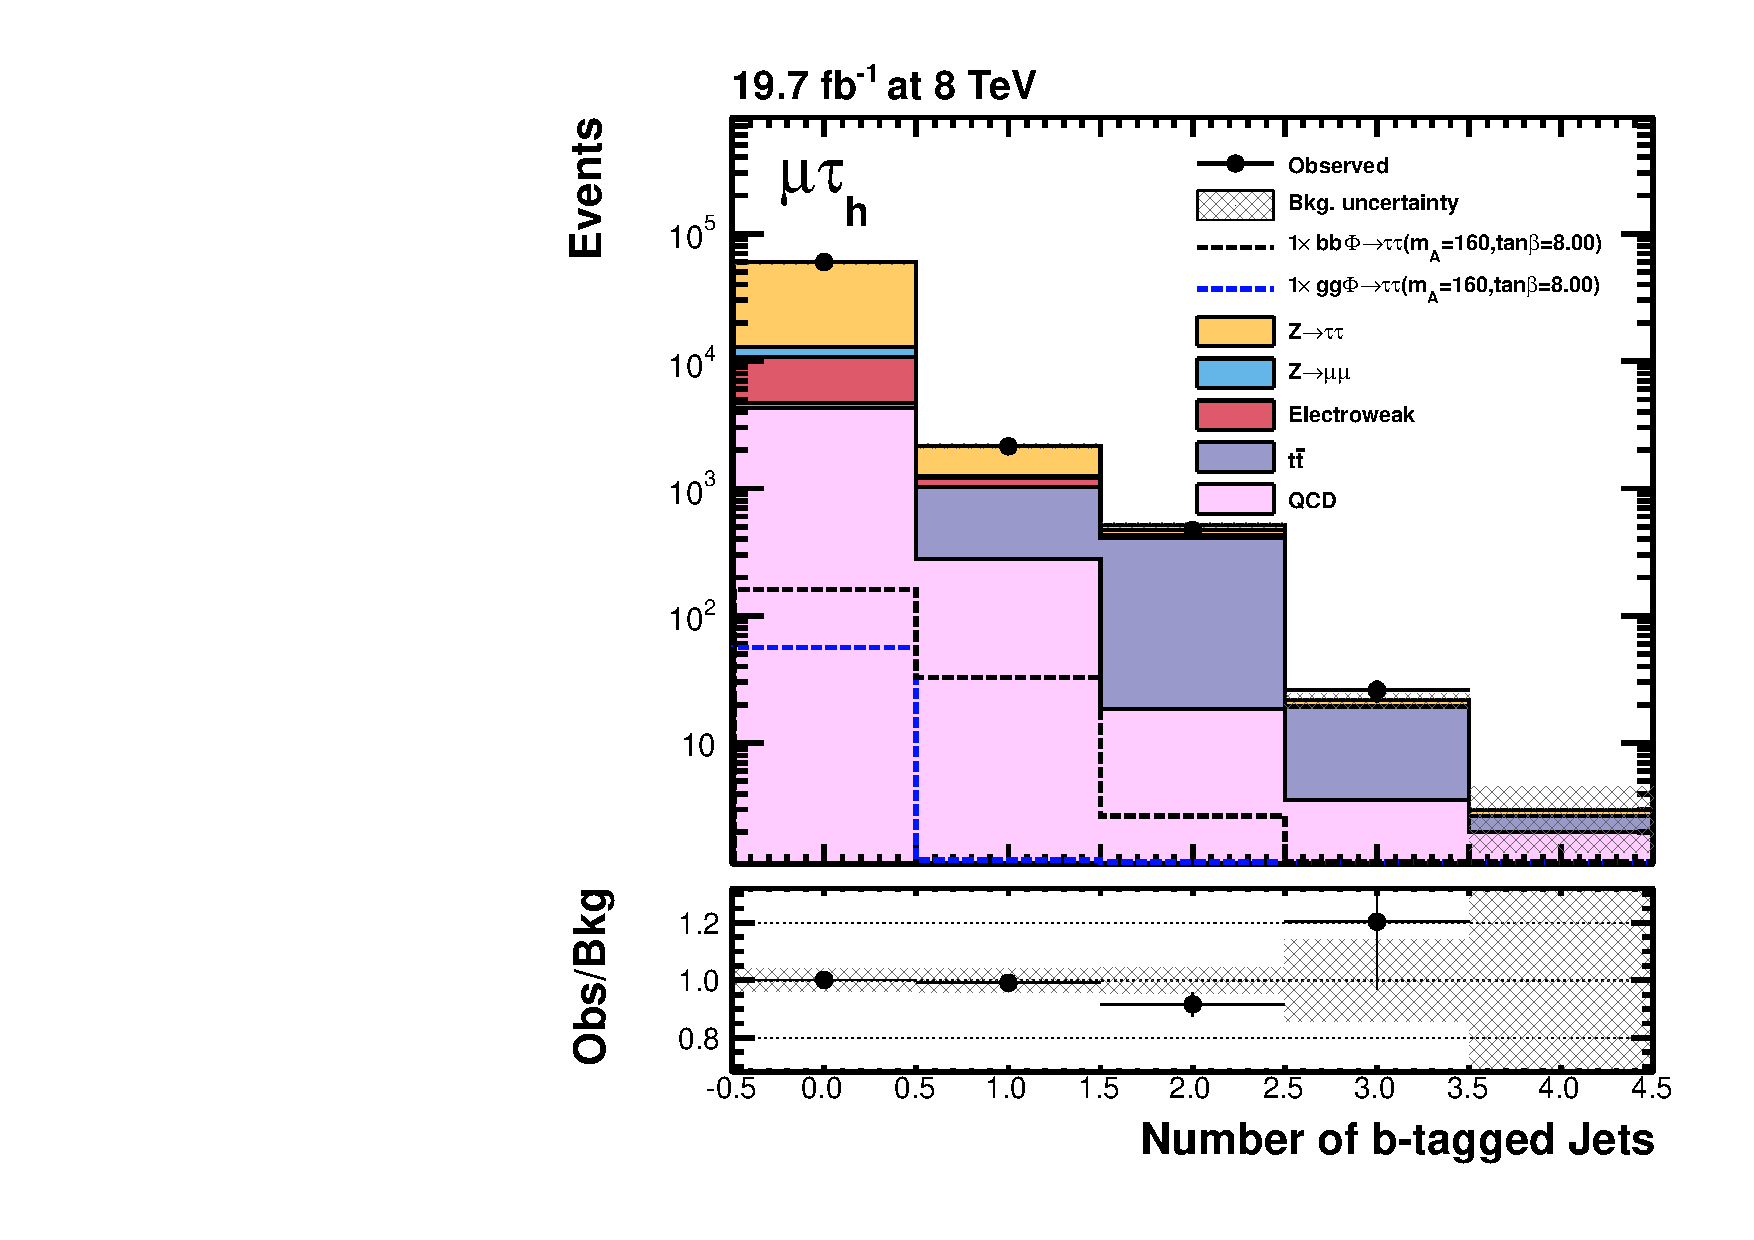
\includegraphics[width=0.6\textwidth]{plots/htt-mssm/n_bjets_inclusive_mt_2012_log.pdf}

\caption[Number of b-tagged jets in events in the $\mutau$ channel, as used to separate
events into b--tag and no b--tag categories.]{Number of b-tagged jets in events
in the $\mutau$ channel, as used to separate
events into b--tag and no b--tag categories. Signal contributions are shown
separately for b-associated production $\Pqb\Pqb\Pphi$ and gluon fusion
$\Pg\Pg\Pphi$, normalised to a benchmark cross-section times branching ratio.}
\label{fig:nbtag}
\end{figure}

\section{Datasets and Monte Carlo samples}
\label{sec:mssmdataandMC}

The datasets in this analysis correspond to all data collected during the 2011
and 2012 running periods of the LHC.
The \ac{MC} samples for each of the background processes are
identical to those described in section \ref{sec:dataandMC} for the \ac{SM}
analysis. The signal samples for the two production processes are
generated using \textsc{pythia}~\cite{Sjostrand:2006za} at \ac{LO}. They both use \textsc{pythia}
for parton showering and hadronisation and \textsc{tauola}~\cite{TAUOLA} for tau
decays. Additional proton-proton collisions to simulate pileup events are added
as they are for the other samples. The signal samples are generated in a mass range from
$90\,\GeV$ up to $1\,\TeV$ in steps of varying size. Cross-sections times
branching ratios for the signal are taken from the \ac{LHCHXSWG}
\cite{LHCHiggsCrossSectionWorkingGroup:2011ti,Dittmaier:2012vm,Heinemeyer:2013tqa}.

\section{Background estimation and systematic uncertainties}
\label{sec:mssmBackgroundsSysts}

\subsection{Background estimation}
\label{sec:mssmBackgrounds}
The background composition is very similar to that of the \ac{SM} $\HToTauTau$
analysis and the methods used to estimate the contributions follow those
described in section \ref{sec:backgrounds}. The requirement of at least one
b-tagged jet in the b-tag category reduces background from $\ZToTauTau$
and increases the contribution of $\ttbar$. As described in section
\ref{sec:backgroundEstimation_Ztautau}, an embedding procedure is used for the
$\ZToTauTau$ estimate, in which $\PZ\to\Pgm\Pgm$ events in data are replaced
with simulated taus. It is known that a small fraction of selected data events
are $\ttbar$ events instead of $\PZ\to\Pgm\Pgm$ events, and hence it is
necessary to calculate this contamination in the b--tag category so as to avoid
double counting of $\ttbar$. The contamination is estimated by running the
embedding procedure on a $\ttbar$ \ac{MC} sample. For the $\etau$ and $\mutau$ channels, this
contamination is around $1.5\%$ of the $\ZToTauTau$ yield, and so the $\ttbar$ yield is reduced
accordingly by $14\%$. The contribution is negligible in the no b--tag category (as well
as in all the categories of the \ac{SM} analysis). 

Similarly to the way cuts on $m_{jj}$ and $|\Delta\eta_{jj}|$ are relaxed to
obtain smooth shapes for the $\WJets$ background in the VBF categories, the
b-tagging working point for the jets is relaxed to the loose \ac{CSV} working point to
obtain the shape for the b--tag category. This is also done for the shape of
the $\PZ\to\ell\ell$ background. For the QCD estimate, the same-sign data is used for
both shape and normalisation in the no b--tag category, whereas for the b--tag
category the shape is taken from anti-isolated same-sign data using again the relaxed
b-tagging working point.

Data to \ac{MC} corrections are the same as those used in the \ac{SM}
$\HToTauTau$ analysis as described in section~\ref{sec:datamcfactors}. An
additional correction is derived for the $\WJets$ background to account for
observed differences in the jet-tau fake-rate at high $\pt$, which in particular
affects the high mass tail of the $\WJets$. This correction is measured in the
$\WJets$ control region using high $m_{\mathrm{T}}$ events. 

\subsection{Tail fitting of backgrounds}
\label{sec:tailfitting}

The largest difference between the \ac{MSSM} $\Pphi\to\Pgt\Pgt$ analysis and the
\ac{SM} $\HToTauTau$ analysis is the fact that Higgs bosons of
masses up to $1\,\TeV$ are considered. This means that events with high $m_{\Pgt\Pgt}$
are used up to $1.5\,\TeV$. In these high mass regions, the
number of events in the backgrounds is greatly reduced, and it becomes more
difficult to obtain smooth background templates. This results in a need for a
large number of bin-by-bin uncertainties like those described in
section~\ref{sec:systematicUncertainties_shape} to cover bins with low
statistics. A better method for dealing with this is to ensure that the bins are
all populated by fitting the template in the high mass region using an analytic
function, and replacing the tail of the distribution with the binned form of the function.

The function used for the fits takes the following form:

\begin{equation}
f = \exp\left(\frac{-m_{\Pgt\Pgt}}{c_{0} + c_{1}\cdot m_{\Pgt\Pgt}}\right) ,
\end{equation}

where $c_{0}$ and $c_{1}$ are free parameters in the fit. The fit is made to
the \ac{MC} in the region $m_{\Pgt\Pgt} > 150\,\GeV$ and then the template is
replaced by the values of the analytical function for this region. To represent
the uncertainty on this high mass fit in the final maximum-likelihood fit for
signal extraction, shape uncertainties are generated corresponding to the 
values of the function for the $\pm1\sigma$ shift in the fit parameters $c_{0}$ 
and $c_{1}$. The values of these uncertainties are the 
eigenvalues of the covariance matrix of the fit. Figure \ref{fig:tailfits} shows
an example of the fit obtained for the \WJets background in the $\mutau$
channel, showing the central fit to the template and the shape nuisances which
are added to the maximum likelihood fit.

\begin{figure}[tbh]
\subfloat[]{
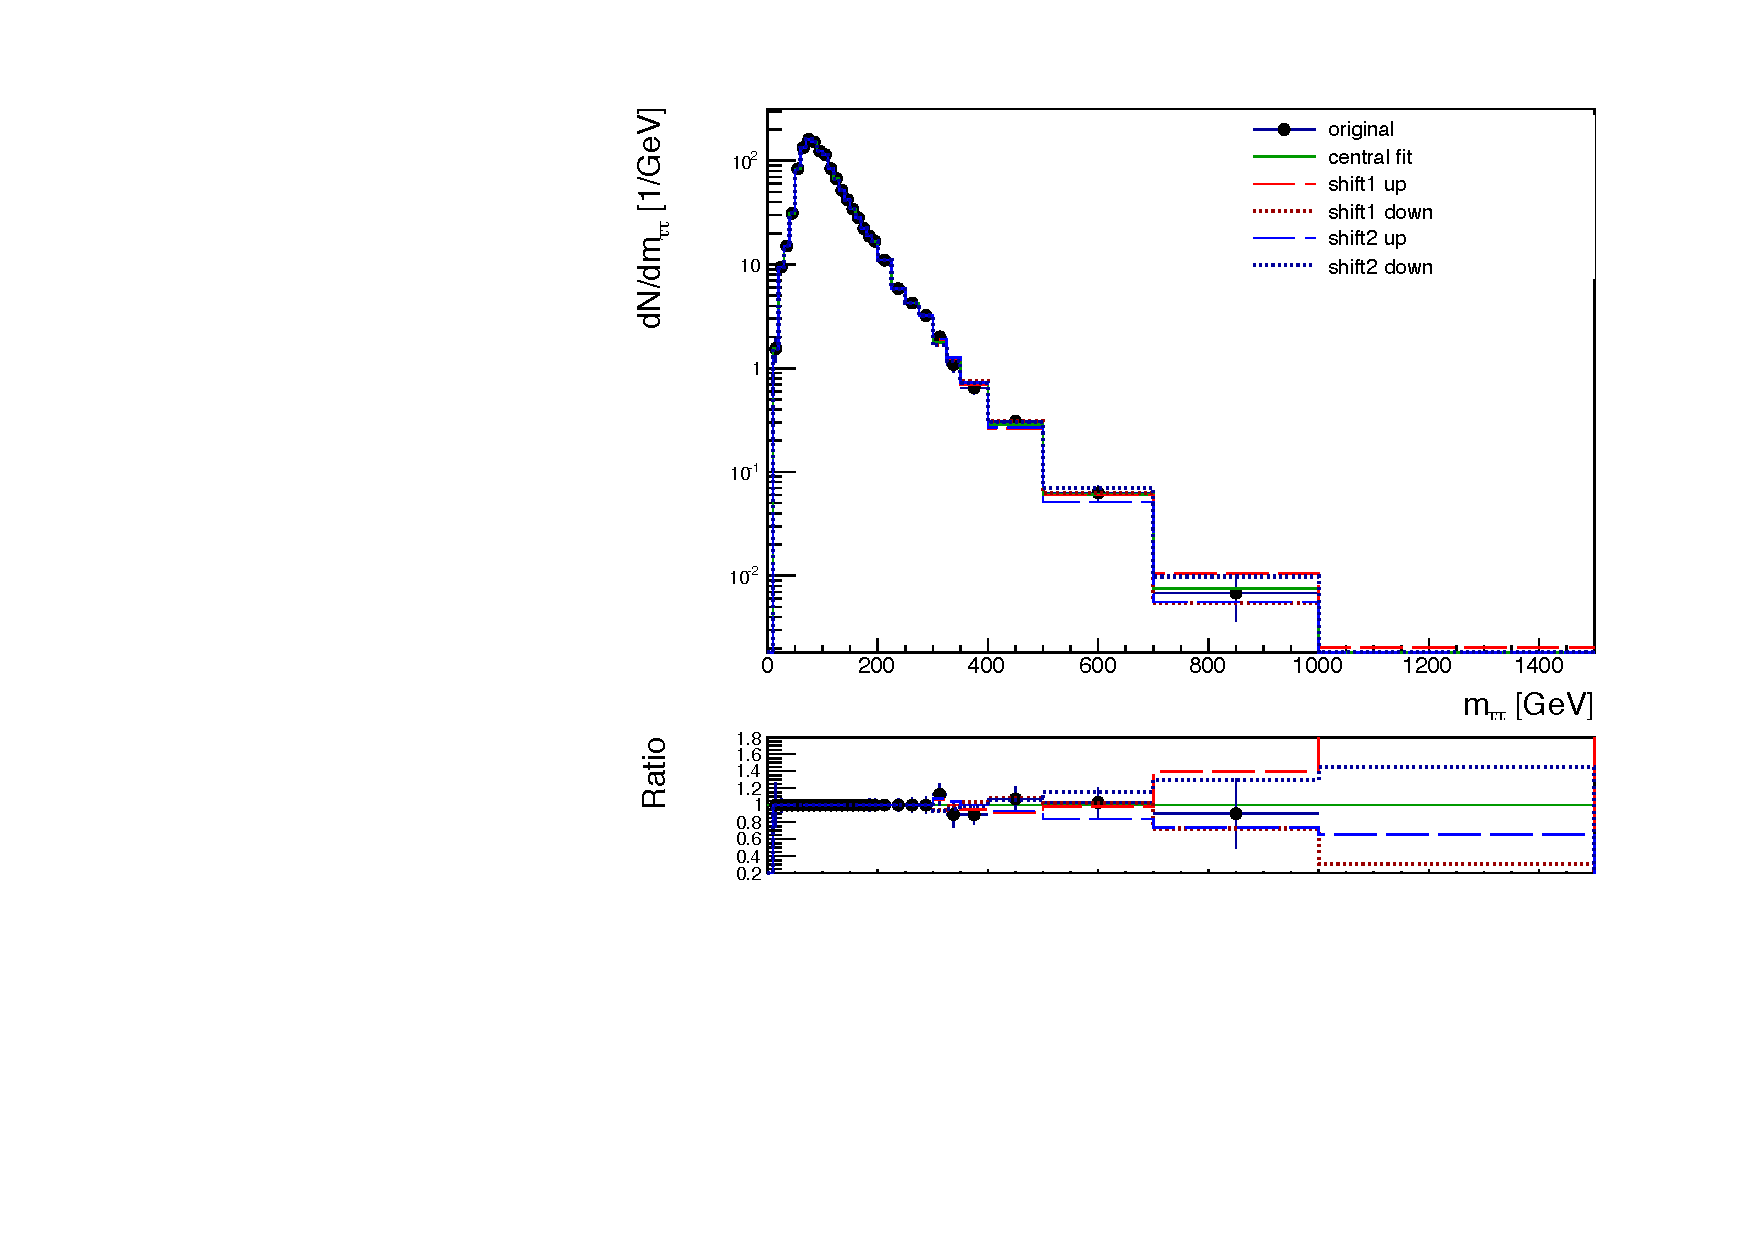
\includegraphics[width=0.5\textwidth]{plots/htt-mssm/W_fine_binning_CMS_shift1_muTau_nobtag_8TeV_Rebin.pdf}}
\subfloat[]{
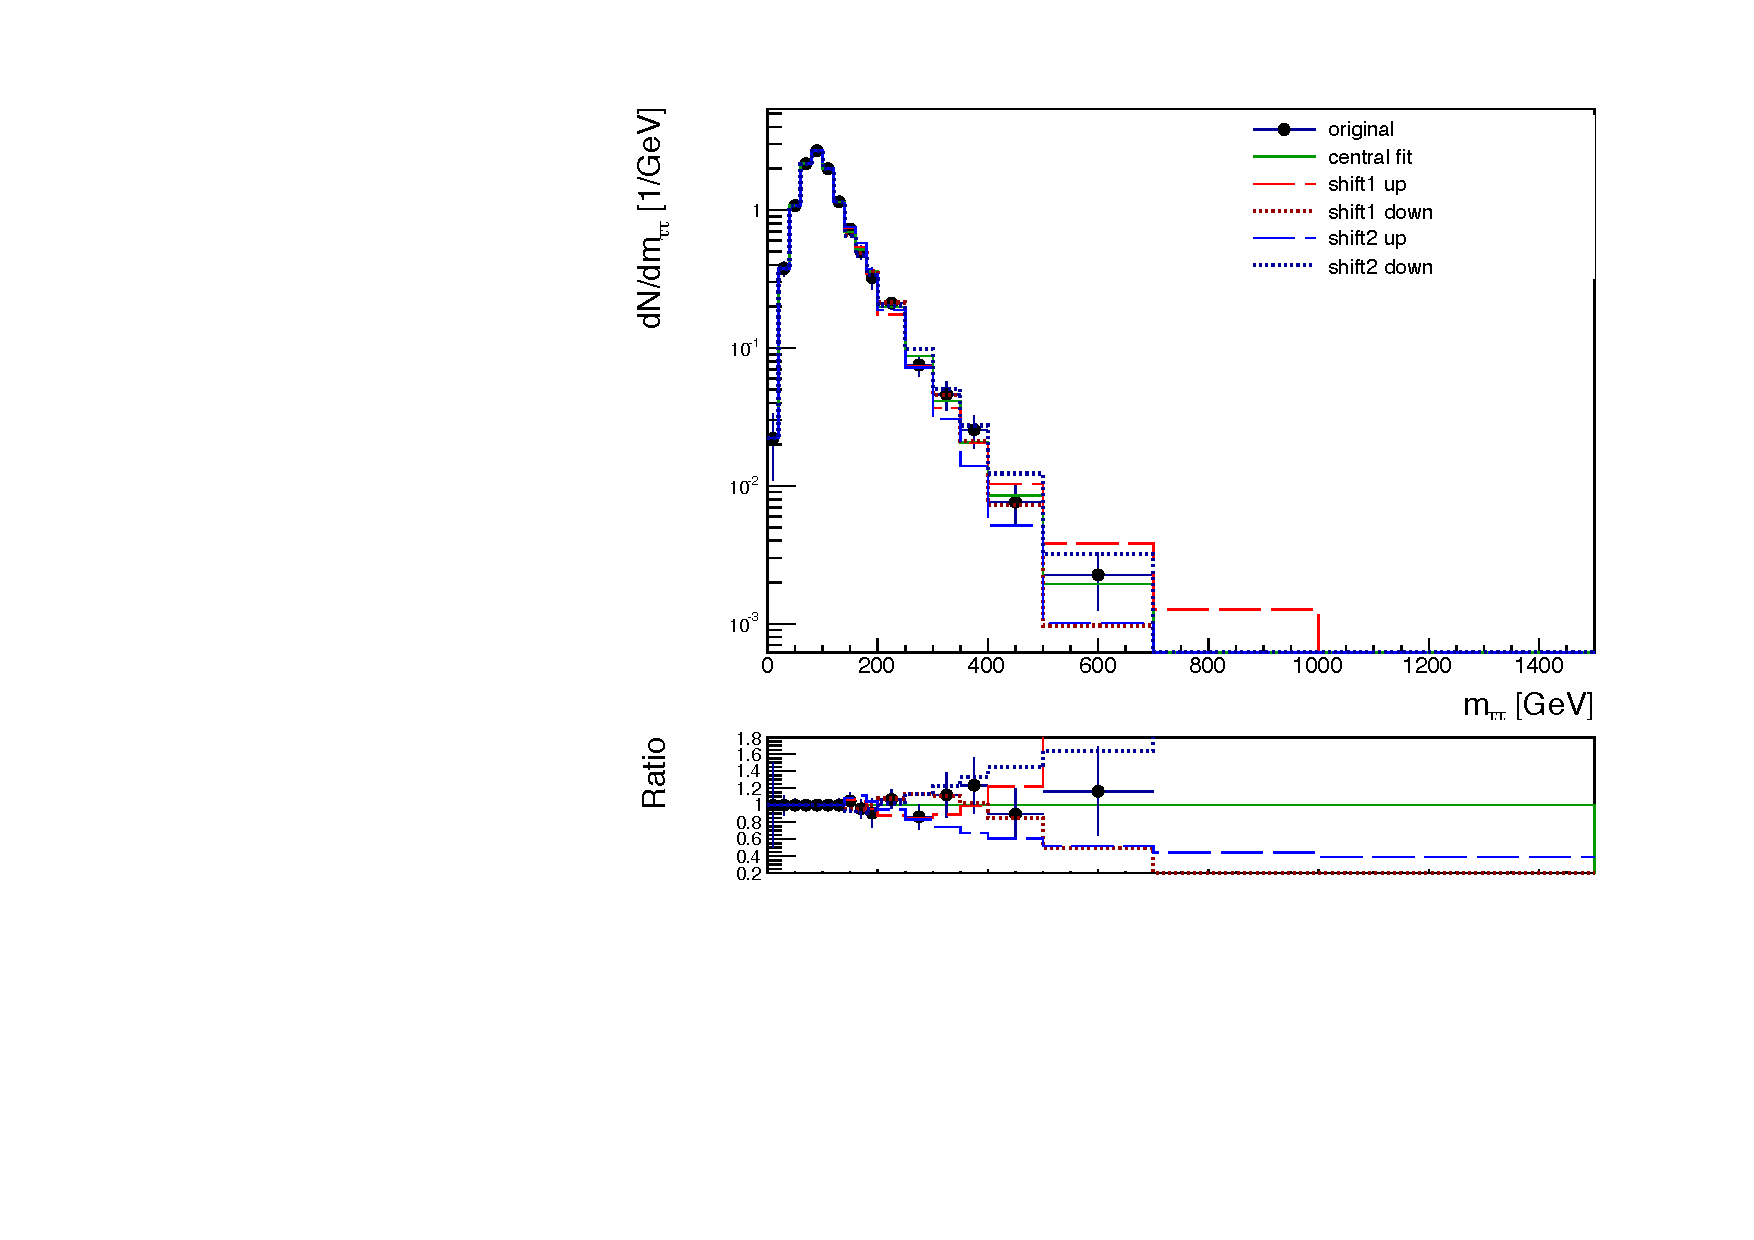
\includegraphics[width=0.5\textwidth]{plots/htt-mssm/W_fine_binning_CMS_shift1_muTau_btag_8TeV_Rebin.pdf}}
\caption[Analytic fits to the high mass tail of the $m_{\Pgt\Pgt}$ distribution,
shown for the example of the $\WJets$ background.]{Analytic fits to the high mass tail of the $m_{\Pgt\Pgt}$ distribution,
shown here for the example of the $\WJets$ background. Fits are shown for the
no b--tag (a) and b--tag (b) categories of the $\mutau$ channel for
$\sqrt{s}=8\,\TeV$. The green line corresponds to the central fit, and the red and blue
lines indicate the systematic uncertainties added to the final
maximum-likelihood fit to propagate through the
uncertainties in the two fitted parameters.}
\label{fig:tailfits}
\end{figure}

Fits are performed for the $\WJets$, QCD, $\ttbar$ and diboson backgrounds in the $\etau$
and $\mutau$ channels, where the statistics in the templates are good enough to
produce a reliable fit. In the backgrounds in which a tail fit is not used, and
in the low mass regions of the fitted backgrounds, bin-by-bin uncertainties as
described in section~\ref{sec:systematicUncertainties_shape} are applied.

\subsection{Other systematic uncertainties}
%%Try to find some references for some of these things
The majority of the systematic uncertainties in the \ac{MSSM} analysis are the
same as those in the \ac{SM} analysis as described in
section~\ref{sec:systematics}. Exactly the same values are taken for ID, isolation and
trigger efficiencies and luminosity uncertainty. Jet and $\MET$ scale
uncertainties are evaluated in the same way as in the \ac{SM} analysis 
for the categories of the \ac{MSSM}. 
Uncertainties due to b-tagging are also evaluated in the same way, 
and are generally larger in the \ac{MSSM} analysis due to
the direct dependence on number of b-tagged jets. The effect of the b--tag scale
factor is to migrate \ac{MC} events between the two categories.

Normalisation uncertainties on the $\ZToTauTau$ background are similar, with the
same $3\%$ cross-section uncertainty and $5\%$ extrapolation uncertainty from
the embedded sample. Uncertainties on $\WJets$ and QCD are calculated
analogously to the \ac{SM} analysis. The same cross-section uncertainties are taken on the $\ttbar$
and diboson backgrounds. The magnitude of the correction to the $\ttbar$ as a result 
of the embedding contamination is taken as an uncertainty in the rate of $\ttbar$ events. A shape 
uncertainty for the correction for jet-tau fake-rate at high $\pt$ on the $\WJets$ background
is also applied, where the shapes are generated by shifting the fake-rate
correction up and down by the uncertainty in its measurement. 

A shape uncertainty to account for tau energy scale is applied in the same way
as the \ac{SM} analysis. Another shape uncertainty is included on the signal to account for differences in tau ID
efficiency at high $\pt$, affecting the high $m_{\Pgt\Pgt}$ events. 
Theoretical uncertainties on the signal are similar to those on the \ac{SM} signal, and vary
with $m_{\PA}$ and $\tan\beta$. The \ac{PDF} uncertainties range from $2$--$10\%$ and scale uncertainties range from
$5$--$25\%$ for gluon-gluon fusion and $8$--$15\%$ for b-associated production
\cite{HIG-13-021}. A summary of all systematics applied in this analysis can be
found in table \ref{tab:MSSMSystematics}.


\begin{table}[tbhp]
\small
\begin{center}
    \begin{tabular}{|l|c|c|c|}
    \hline
    \multicolumn{2}{|c|}{Source of uncertainty}
    & \multicolumn{2}{|c|}{Event yield uncertainty}  \\
    \multicolumn{2}{|c|}{and affected processes} & \multicolumn{2}{|c|}{by event category} \\
    \hline
     Experimental uncertainty                                  & Affected processes &  no b--tag     &  b--tag      \\
     \hline
     Integrated lumi. $7/8\,\TeV$                           & All MC & 2.2/2.6\% & 2.2/2.6\%       \\
     \Pe ID \& trigger                                   & All MC &  2\%  & 2\%       \\
     \Pmu ID \& trigger                                       & All MC & 2--3\%       &   2--3\%        \\
     \Pgt ID \& trigger                                        & All MC & 8\%, shape  & 8\%, shape           \\
     b-tag efficiency                                      & All MC & 1--5\% & 1--6\%  \\
     b-mistag rate                                             & All MC & 1--3\% & 2--9\%    \\
     \hline
     $\PZ$ production                                          & $\ZToTauTau$, $\PZ\to\ell\ell$ & 3.3\%     &   3.3\%      \\
     $\PZ\to\Pgt\Pgt$: category selection                      & $\ZToTauTau$ & -  & 3\%        \\
     $\PZ\to\Pgt\Pgt$: $\ttbar$ contamination                  & $\ttbar$ & - & 14\%  \\
     Norm. $\ttbar$                                            & $\ttbar$ & 10\%  & 10\%        \\
     Norm. di-boson                                            & diboson & 15\%  &  15\%      \\
     Norm. QCD                                                 & QCD  & 10\%    &   20\%         \\
     Norm. $\WJets$                                            & $\WJets$ & 10\% &  30\%              \\
     $\Pe$ misid. as $\Pgth$                            & $\PZ\to\Pe\Pe$ & 30\%   & 30\%      \\
     $\Pgm$ misid. as $\Pgth$                           & $\PZ\to\Pmu\Pmu$ & 30\%  & 30\%         \\
     Jet misid. as $\Pgth$                              & $\PZ\to\ell\ell$, $\WJets$ & 20\%, shape & 20\%, shape             \\
     \hline
     Tau energy scale                                          & $\ZToTauTau$, signal  & 2--4\%, shape & 2--4\%, shape  \\
     Jet energy scale                                          & All MC & 1\%  &   1-11\%         \\
     \MET scale                                                & All MC & 1\% &   1\%       \\
     \hline
     PDF                                 & signal                                   & 2--10\%   & 2--10\%   \\
     Scale variation (gluon fusion)      & signal                                   & 5--25\%   & 5--25\%   \\
     Scale variation (b-associated)      & signal                                   & 8--15\%   & 8--15\%   \\
    \hline
    Limited bin statistics              & all                                       & shape     & shape     \\
    High-$m_{\Pgt\Pgt}$ tail fit                & QCD, $\ttbar$, $\WJets$, diboson          & shape   & shape     \\
    \hline
     \end{tabular}
    \caption[Systematic uncertainties that affect the estimated number of signal or
    background events in the MSSM $\Pphi\to\Pgt\Pgt$ analysis.]{
    Systematic uncertainties that affect the estimated number of signal or
    background events. Several uncertainties are treated as correlated for the
    different decay channels and event categories. Some uncertainties vary
    across final states and for different affected processes, so ranges are given. 
    Adapted from \cite{HIG-13-021}.}
     \label{tab:MSSMSystematics}
     \end{center}
\end{table}


\section{Results}
\label{sec:mssmresults}

\subsection{Signal extraction}
\label{sec:mssmSignalExtraction}

The discriminating variable used for signal extraction is the same as in the
\ac{SM} analysis - the di-tau mass $m_{\Pgt\Pgt}$, using values up $1.5\,\TeV$.
The maximum likelihood fit is performed using similar methods to those described in 
section~\ref{sec:signalextraction}, using a simultaneous fit to all channels and
categories as described by equations~\ref{eq:LikelihoodFunction} and \ref{eq:PoissonDistribution}.

Figure~\ref{fig:mssmpostfitmass} shows the post-fit di-tau mass distribution in the
$\etau$ and $\mutau$ channels for the b--tag and no b--tag categories. The plots
are shown on a logarithmic scale to highlight the tail of the distribution, of
interest in the \ac{MSSM} analysis. The signal shown is for a benchmark cross
section times branching ratio and combines the two signal production processes
and all three neutral Higgs bosons. No excess of events in data is seen compared 
with the prediction from backgrounds.

\begin{figure}[tbh]
\subfloat[]{
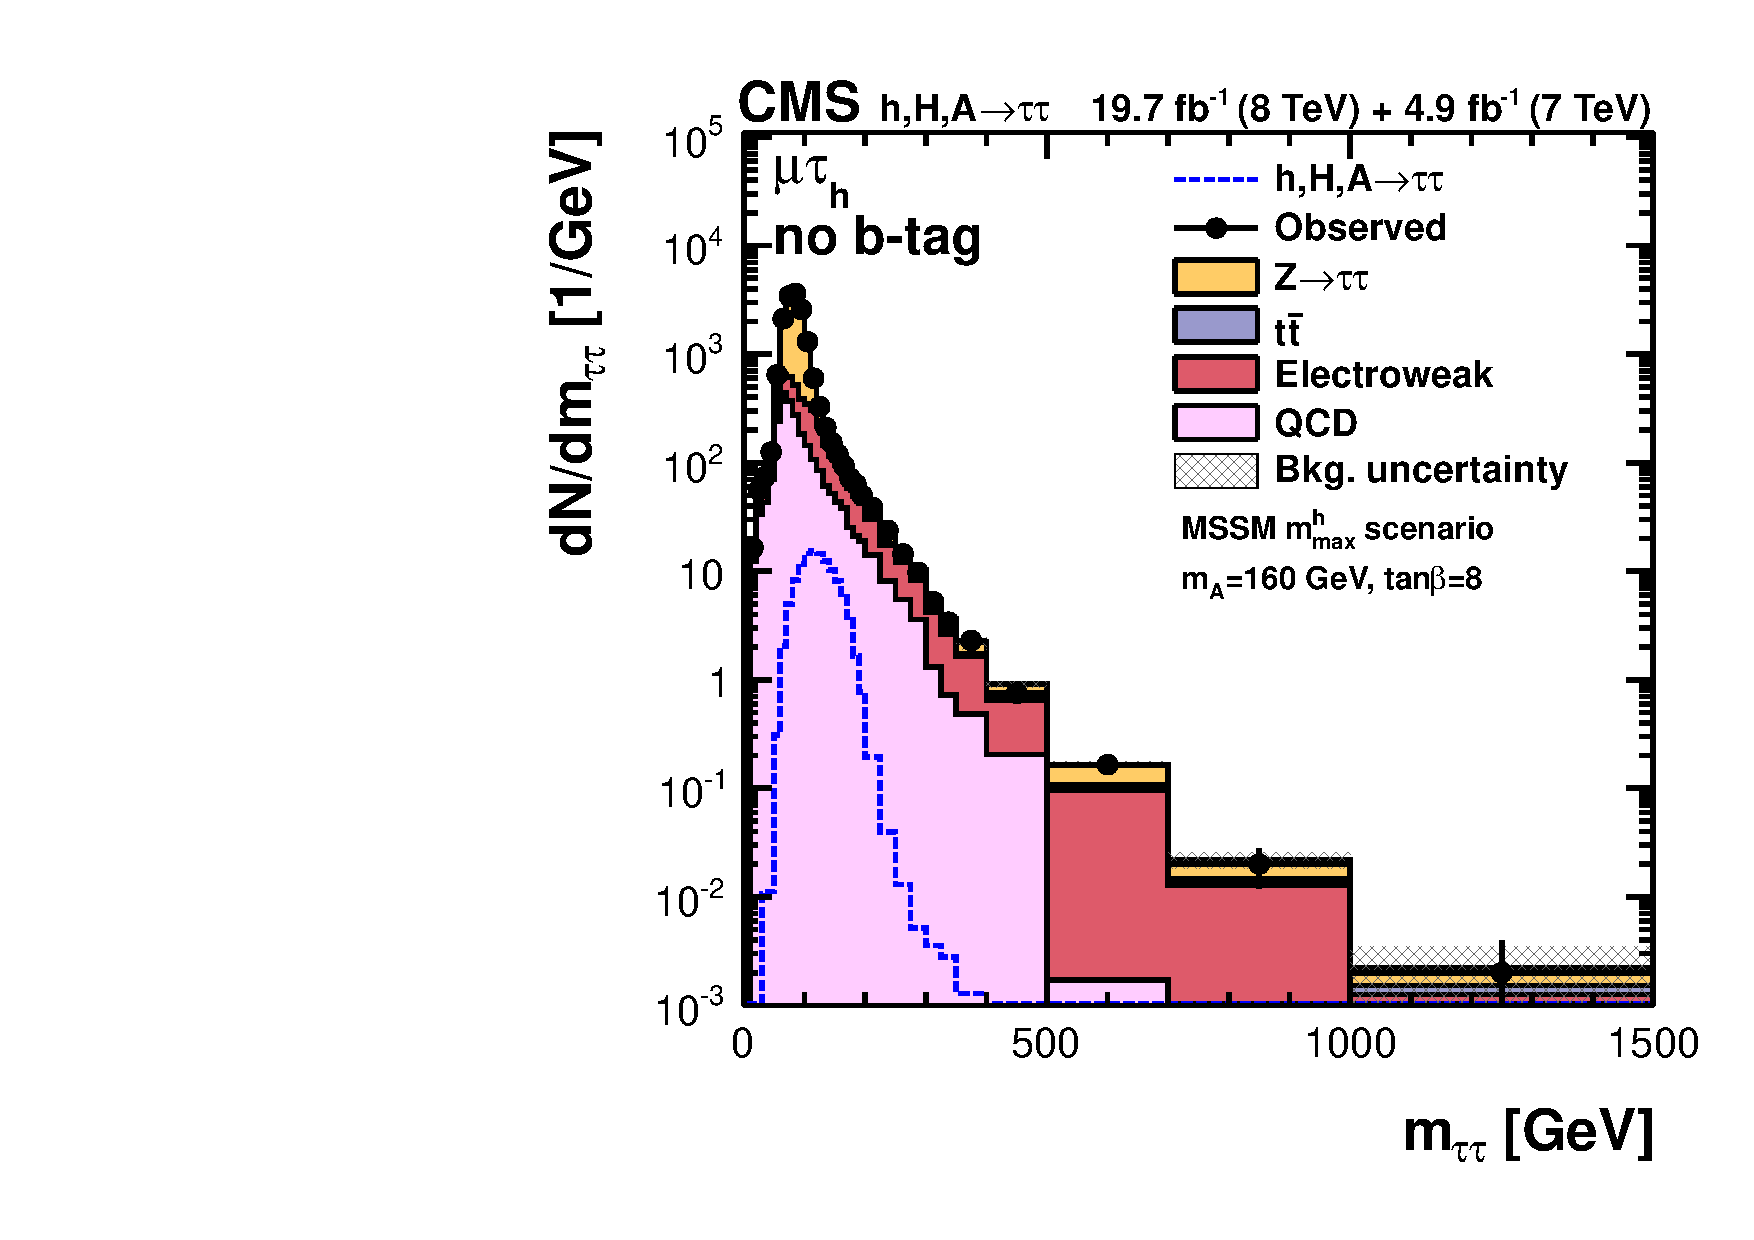
\includegraphics[width=0.5\textwidth]{plots/htt-mssm/muTau_nobtag_postfit_7TeV_8TeV_LOG.pdf}}
\subfloat[]{
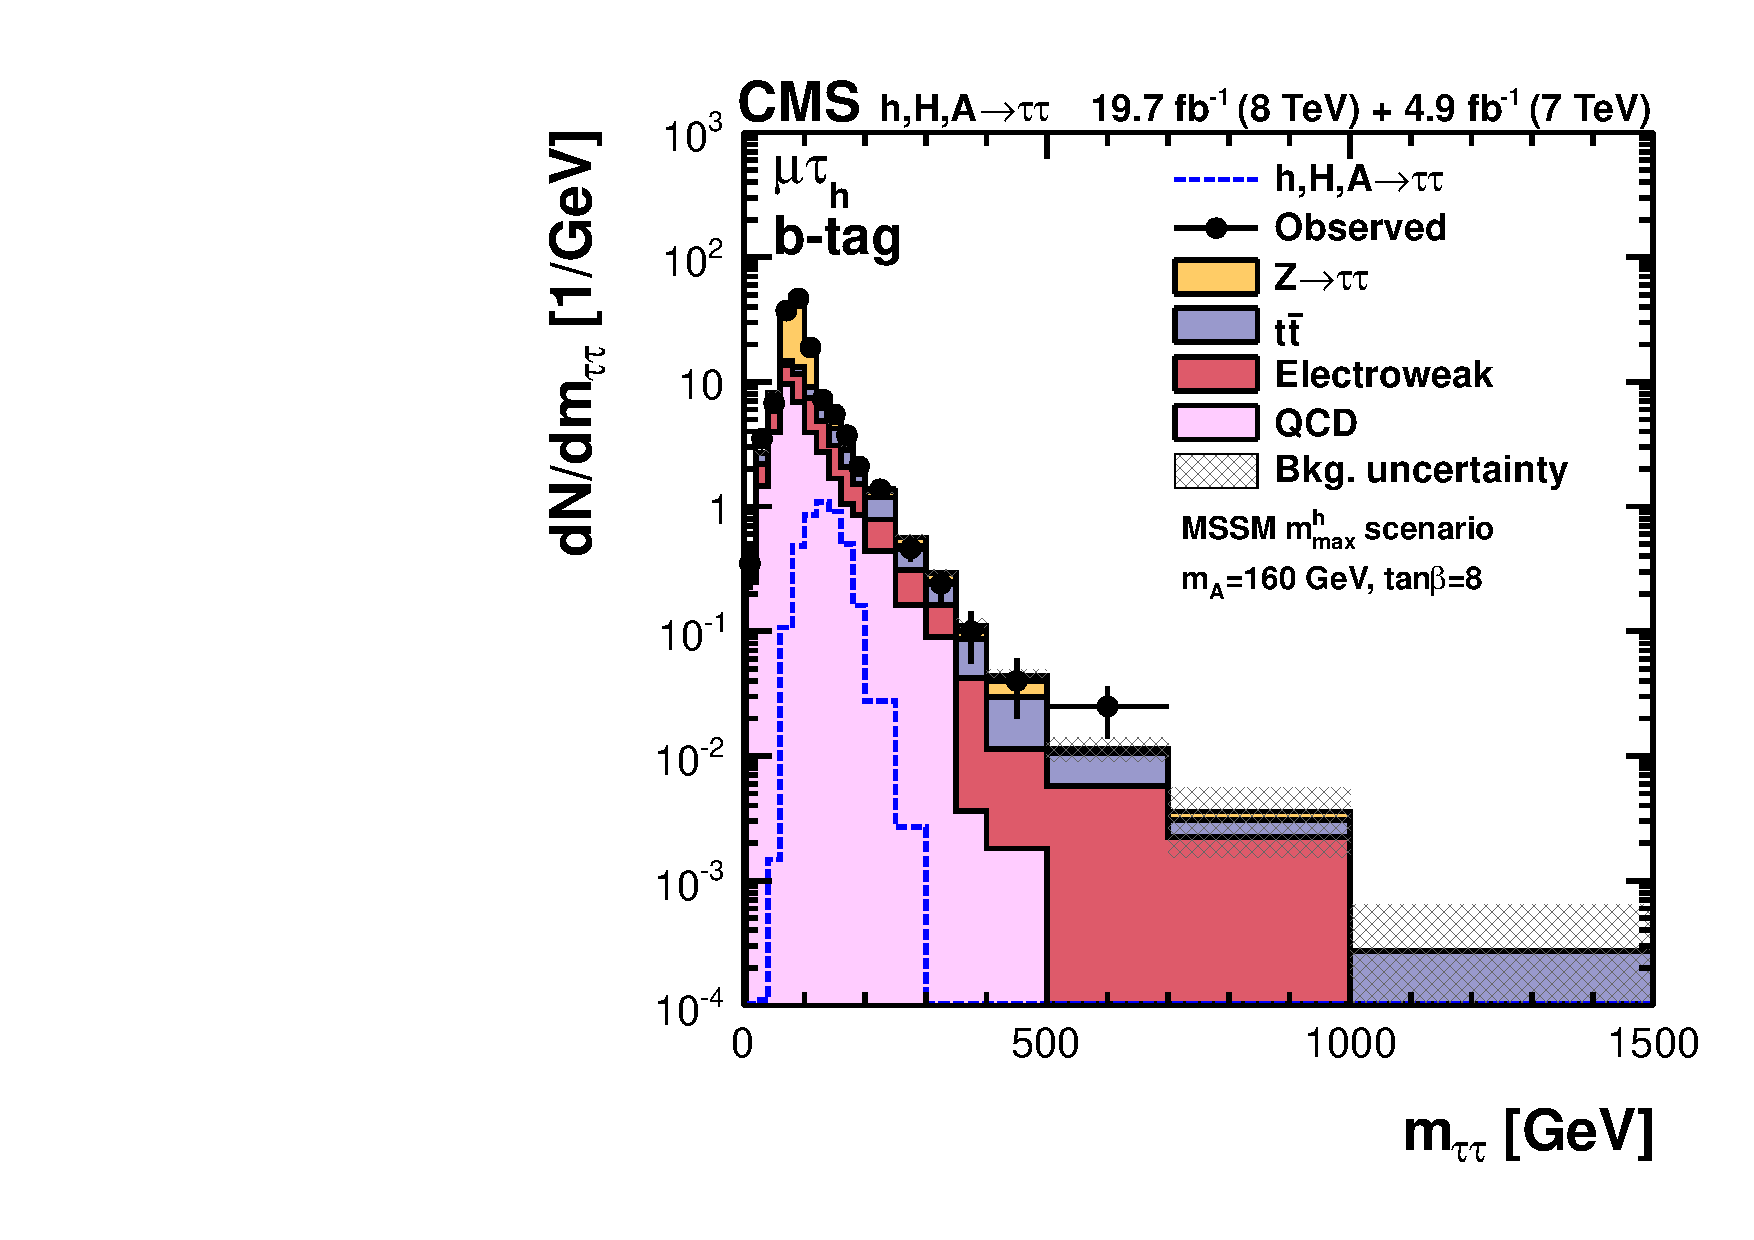
\includegraphics[width=0.5\textwidth]{plots/htt-mssm/muTau_btag_postfit_7TeV_8TeV_LOG.pdf}}

\subfloat[]{
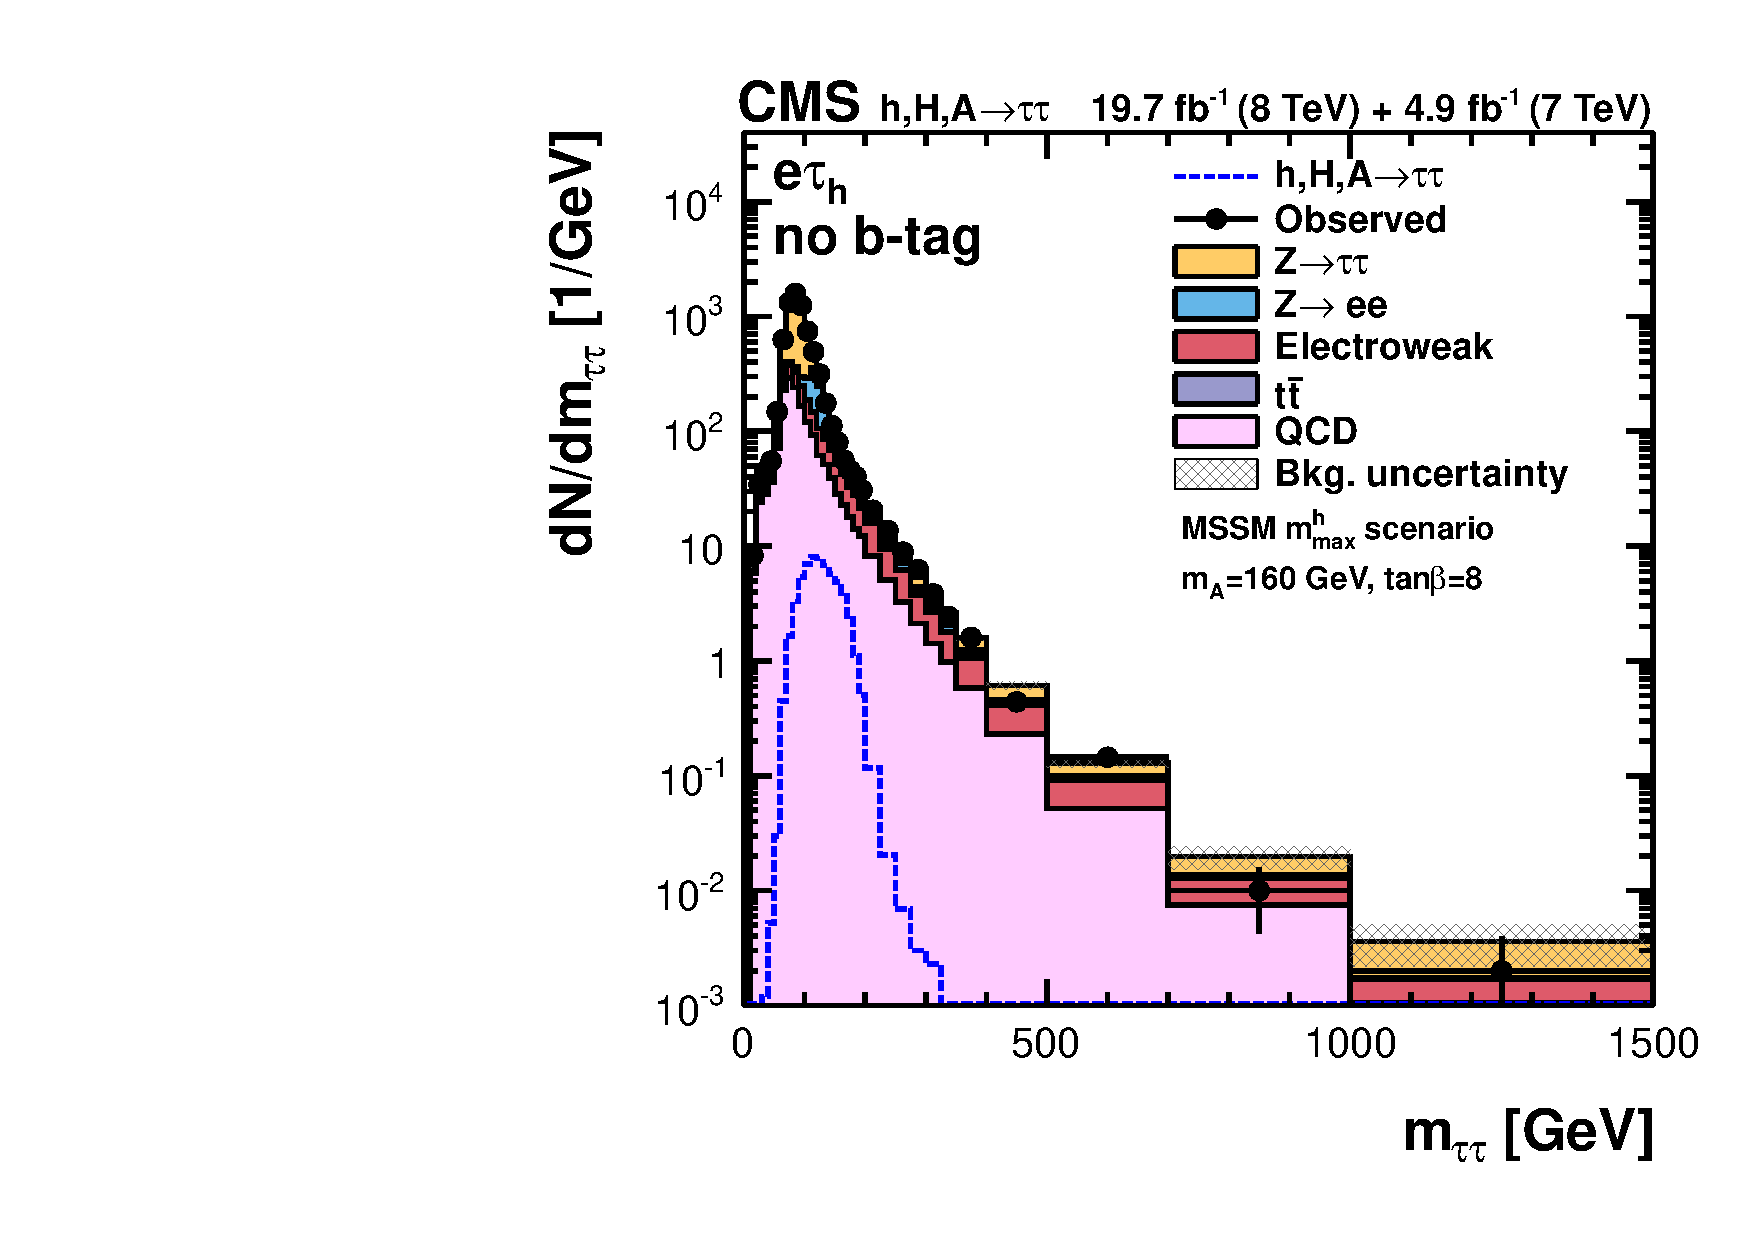
\includegraphics[width=0.5\textwidth]{plots/htt-mssm/eleTau_nobtag_postfit_7TeV_8TeV_LOG.pdf}}
\subfloat[]{
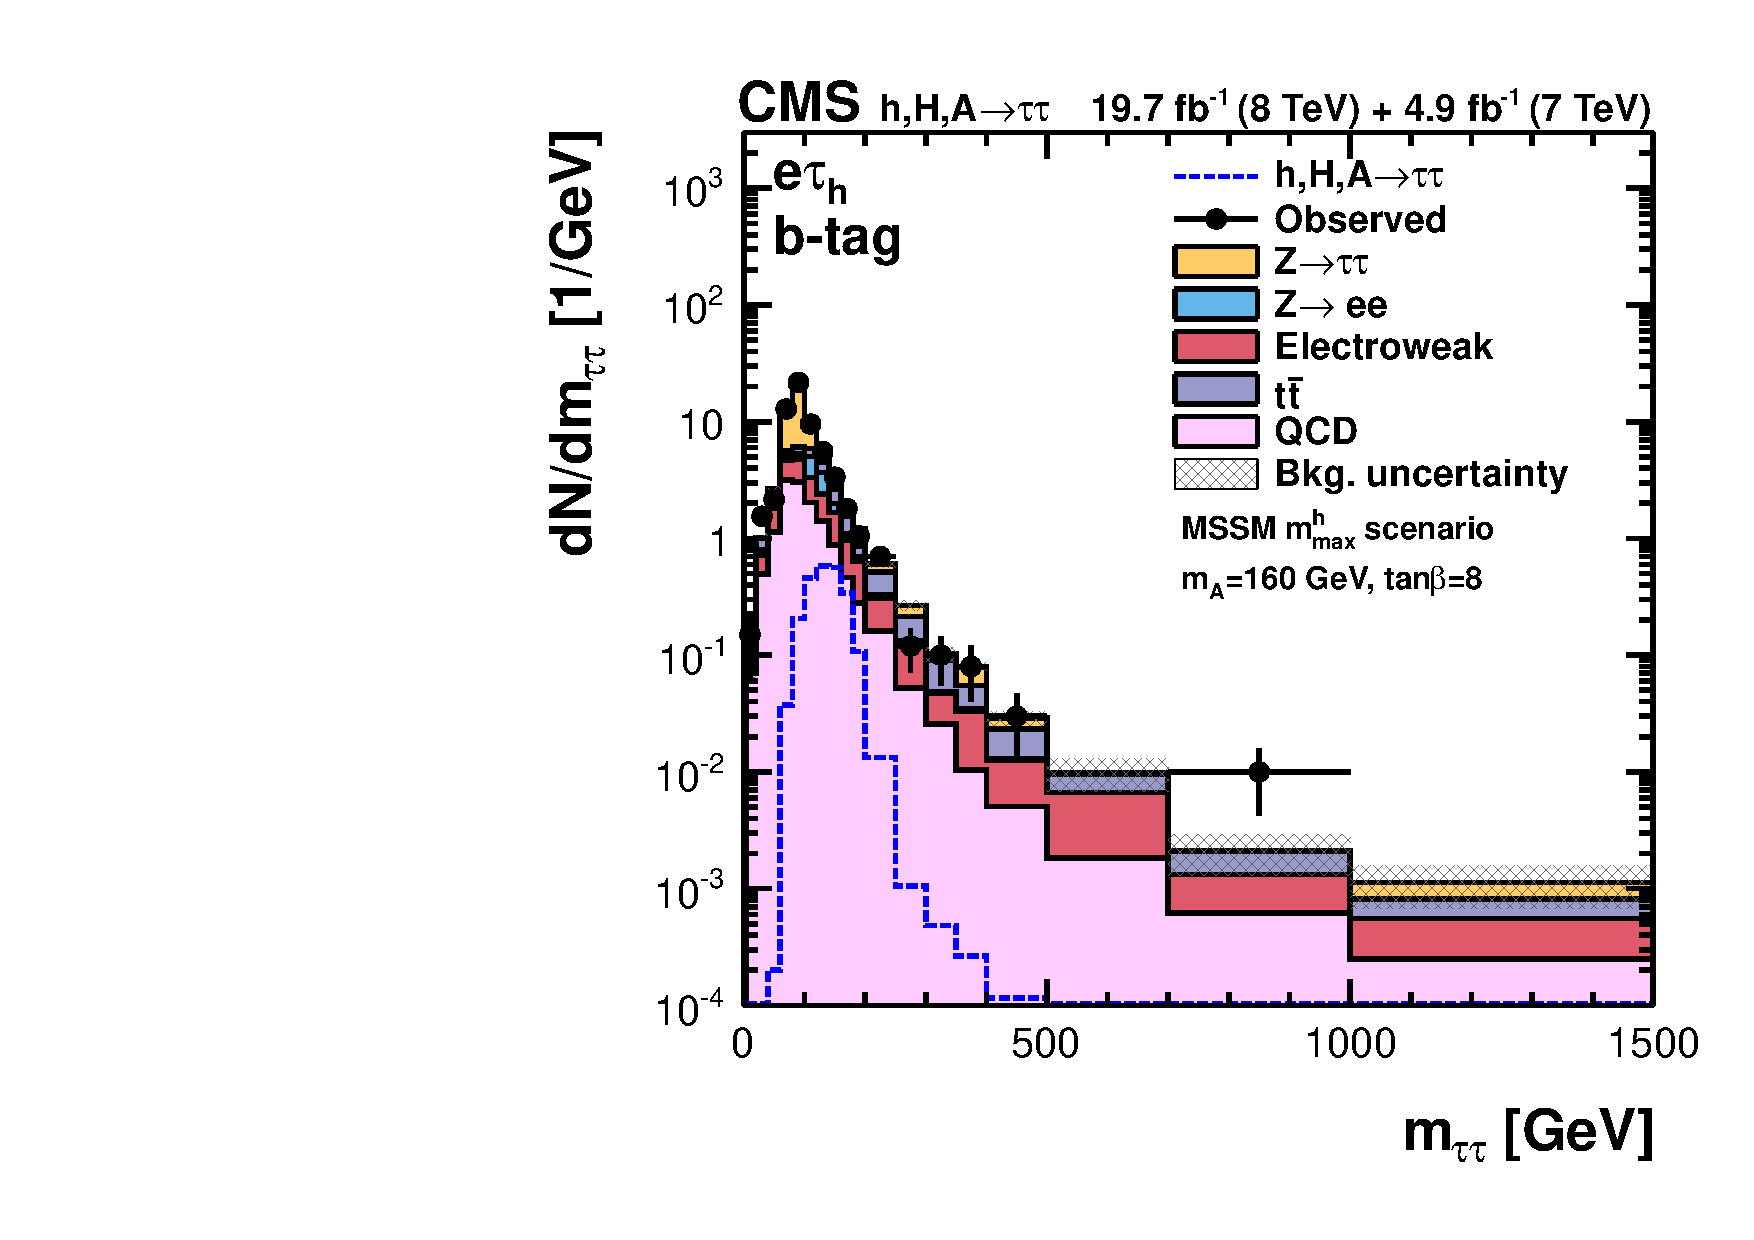
\includegraphics[width=0.5\textwidth]{plots/htt-mssm/eleTau_btag_postfit_7TeV_8TeV_LOG.pdf}}
\caption[Post-fit $m_{\Pgt\Pgt}$ distributions for the no b--tag
and b--tag categories.]{Post-fit $m_{\Pgt\Pgt}$ distributions for the no b--tag
(left) and b--tag (right) categories. Plots are shown for
the $\mutau$ channel (top) and $\etau$ channel (bottom), for the combination of
$7$ and $8\,\TeV$ data \cite{HIG-13-021}.}
\label{fig:mssmpostfitmass}
\end{figure}

The \ac{MSSM} analysis differs from the \ac{SM} analysis in the
interpretation of the results of the maximum likelihood fit in the form of a limit. This
is done differently for the two types of result produced - referred to as `model 
independent' and `model dependent'. 

\subsection{Model independent results}
\label{sec:modelindependent}

\subsubsection{2D likelihood scan}

As discussed in section~\ref{sec:signalextraction}, the maximum-likelihood fit
is generally performed in the signal plus background hypothesis, allowing the
signal to float as controlled by the signal strength modifier $\mu$. In the
\ac{SM} analysis the contributions from all different types of \ac{SM} Higgs
signal: gluon fusion, \ac{VBF} and associated production, are controlled by the
same $\mu$ which is normalised to the \ac{SM} prediction for cross-section times
branching ratio of each process. For the \ac{MSSM}
analysis there are many alternative predictions for the cross-section times
branching ratio for each of the two production processes: gluon fusion and
b-associated production, dependent on the choice of the parameters of the
\ac{MSSM} model. Hence the maximum likelihood fit can be used to obtain the best
choice of cross-section times branching ratio for each of the two production
processes from the fit to data, by letting them both float independently,
without any necessary choice of \ac{MSSM} model.

The signal prediction is defined as follows:
\begin{equation}
\mu \cdot s(\theta) = \mu_{\Pg\Pg\Pphi} \cdot s_{\Pg\Pg\Pphi}(\theta) + \mu_{\Pqb\Pqb\Pphi}
\cdot s_{\Pqb\Pqb\Pphi}(\theta) ,
\end{equation}

where $s_{\Pg\Pg\Pphi}(\theta)$ and $s_{\Pqb\Pqb\Pphi}(\theta)$ are the signal expectations for the gluon
fusion and b-associated production process and $\mu_{\Pg\Pg\phi}$ and
$\mu_{\Pqb\Pqb\phi}$
the signal strength modifiers corresponding to the cross-section times branching
ratio of each process. This can be directly inserted into the likelihood
term defined in equation~\ref{eq:LikelihoodFunction} to obtain a modified
likelihood which depends on two signal strength modifiers instead of one. A
likelihood scan is performed, restricting the signal strength modifiers to
be positive, in steps of cross-section times branching ratio in picobarns. For
each point in the 2-D plane of the two signal strength modifiers, the negative
log likelihood, defined as:
\begin{equation}
\mathrm{NLL} = - \ln \mathcal{L} ,  
\end{equation}
is evaluated. The lowest value of $\mathrm{NLL}$ in the 2D plane is the best fit value
for the two signal strength modifiers. The one and two sigma contours are
calculated as the points $x$ in the plane where:

\begin{equation}
\Delta(\mathrm{NLL})_{1\sigma} = \mathrm{NLL}(\text{best fit}) - \mathrm{NLL}(x) = 0.5 ,\\ 
\Delta(\mathrm{NLL})_{2\sigma} = \mathrm{NLL}(\text{best fit}) - \mathrm{NLL}(x) = 1.92 , 
\end{equation}

where $\mathrm{NLL}(\text{best fit})$ is the lowest $\mathrm{NLL}$ value in the plane and the
values of 0.5 and 1.92 correspond to the 68\% and 95\% confidence intervals
respectively.

A likelihood scan is performed for each mass hypothesis $m_{\Pphi}$. 
This type of result is referred to as a `single-resonance' search,
due to the fact that there is no requirement that the three Higgs bosons of the
\ac{MSSM} are included, the search is simply for the production of $\Pphi$,
which represents any of the three bosons. Figure \ref{fig:2Dlikelihood} shows the 
result for four example $m_{\Pphi}$ values across the. 
The best fit point is indicated by a black cross and the 1 and 2 $\sigma$
contours are shown. The fit result is compared with the result obtained in the
case where an \ac{SM} Higgs is in our dataset and no \ac{MSSM} Higgs is present
- this indicates that a small positive value of cross-section times branching
ratio for the gluon fusion production mode can be obtained as a result of the
\ac{SM} gluon fusion production. Consideration of the effect of a possible
\ac{SM} Higgs on the results of the \ac{MSSM} analysis is discussed further in
the next sections.

\begin{figure}[tbh]
\subfloat[]{
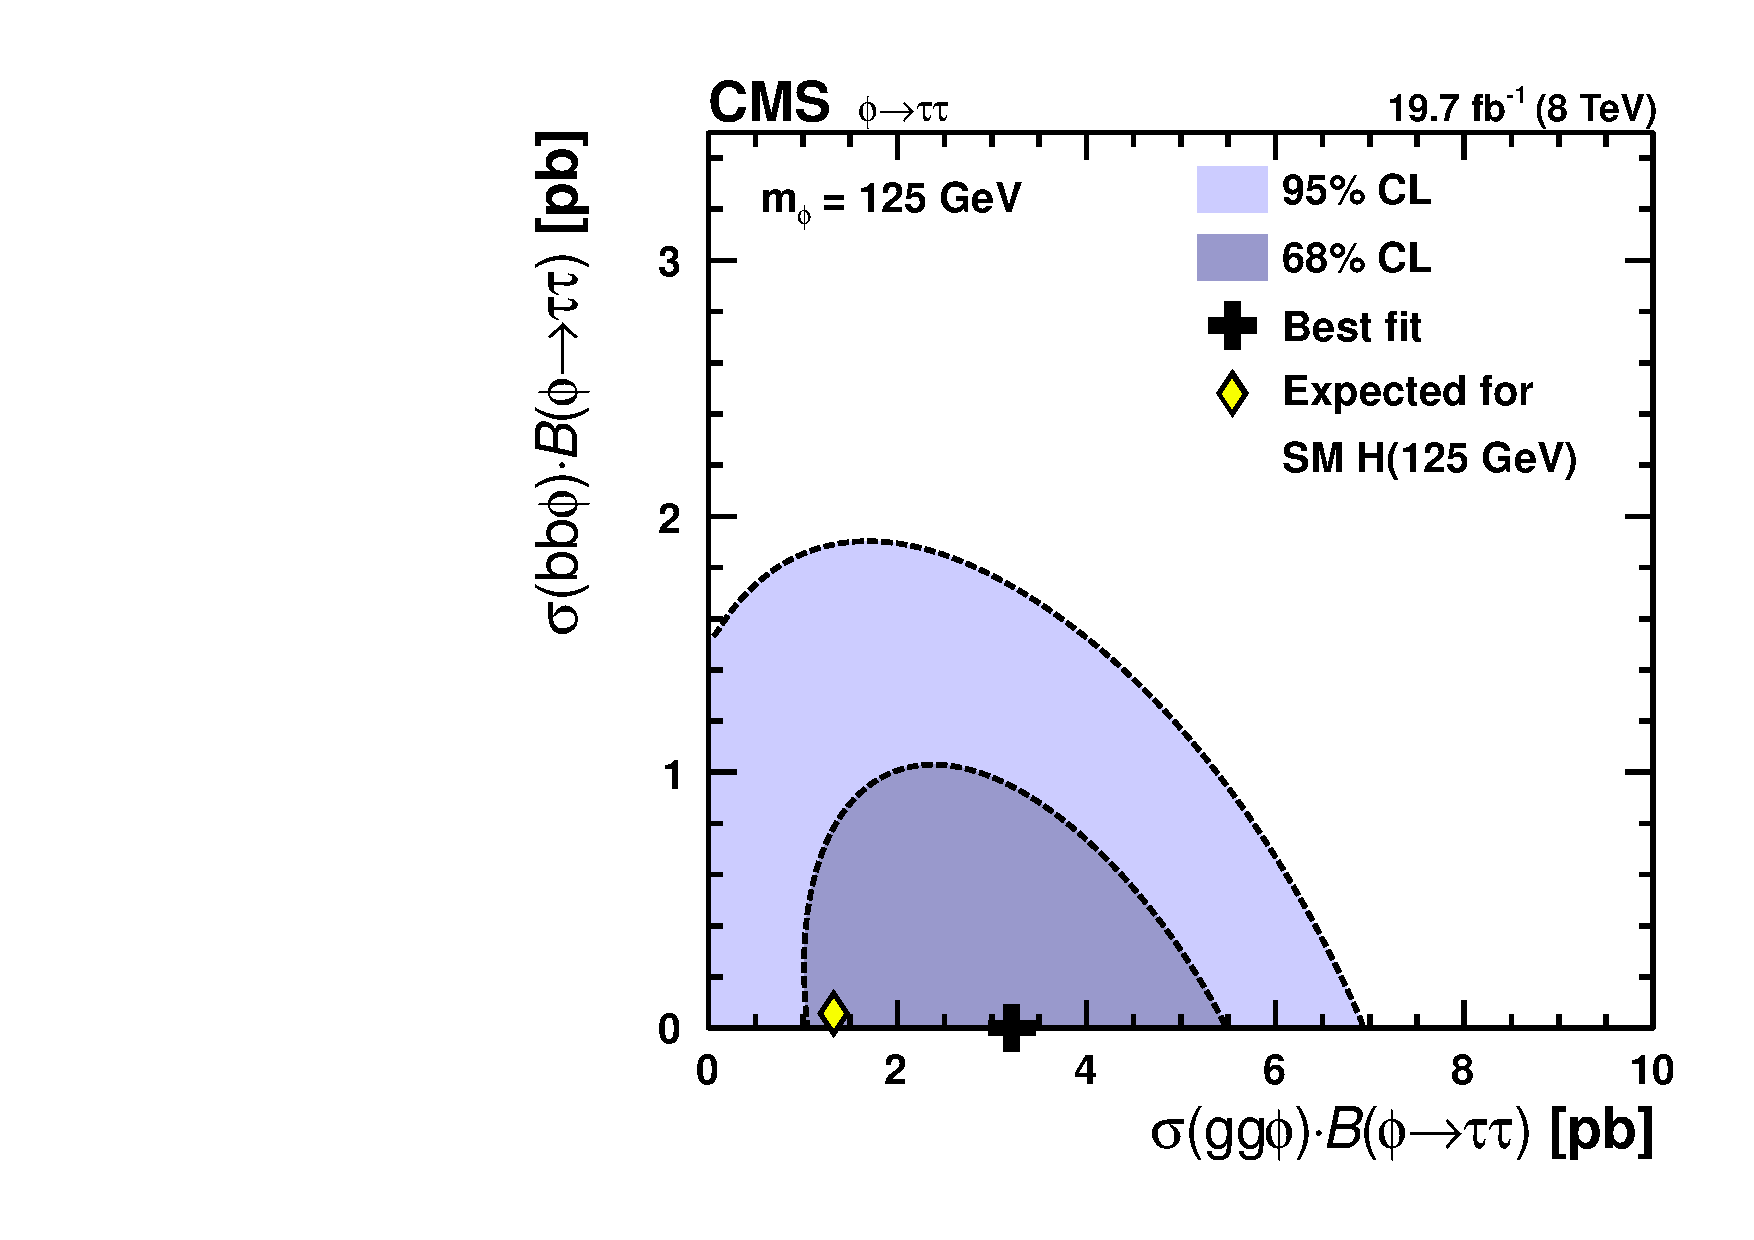
\includegraphics[width=0.5\textwidth]{plots/htt-mssm/bbb-ggH-bbH-scan-GGH-BBH-125.pdf}}
\subfloat[]{
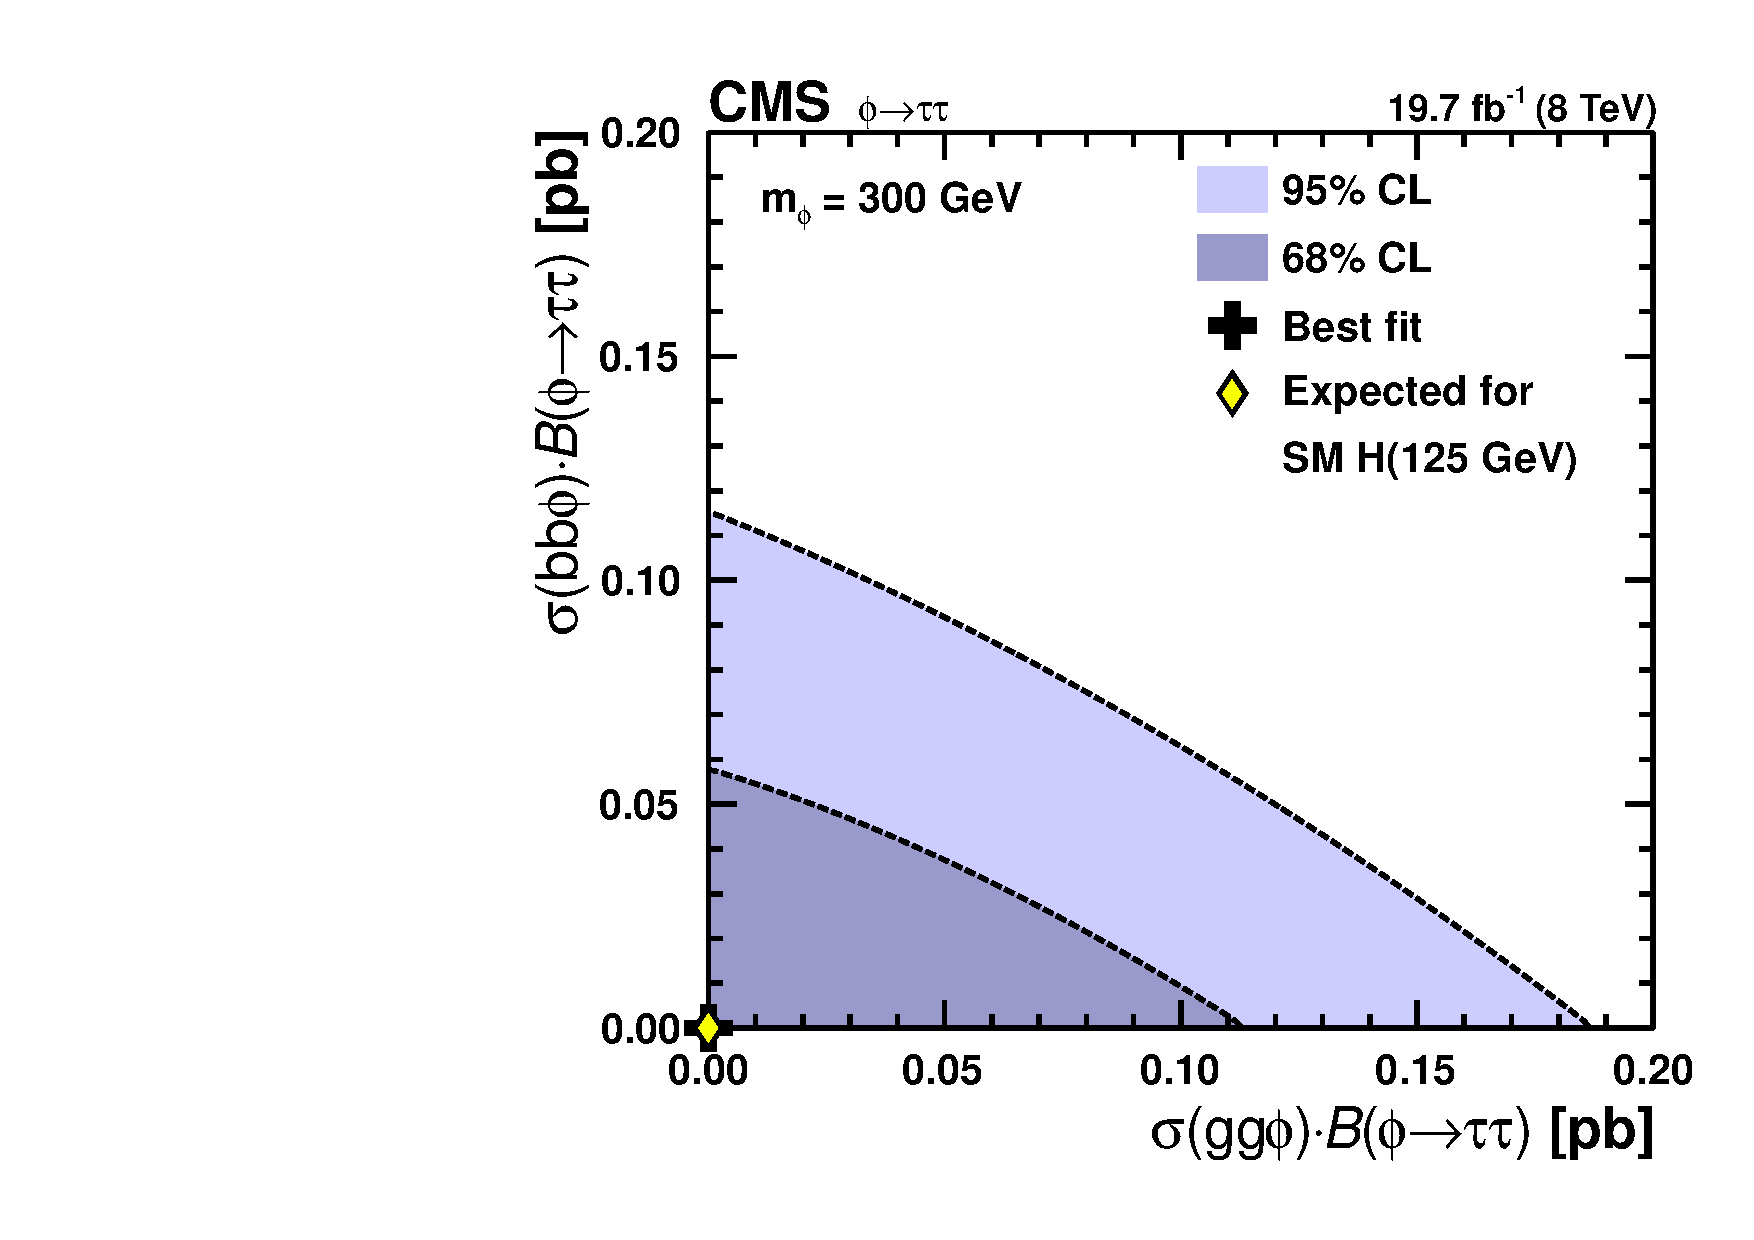
\includegraphics[width=0.5\textwidth]{plots/htt-mssm/bbb-ggH-bbH-scan-GGH-BBH-300.pdf}}

\subfloat[]{
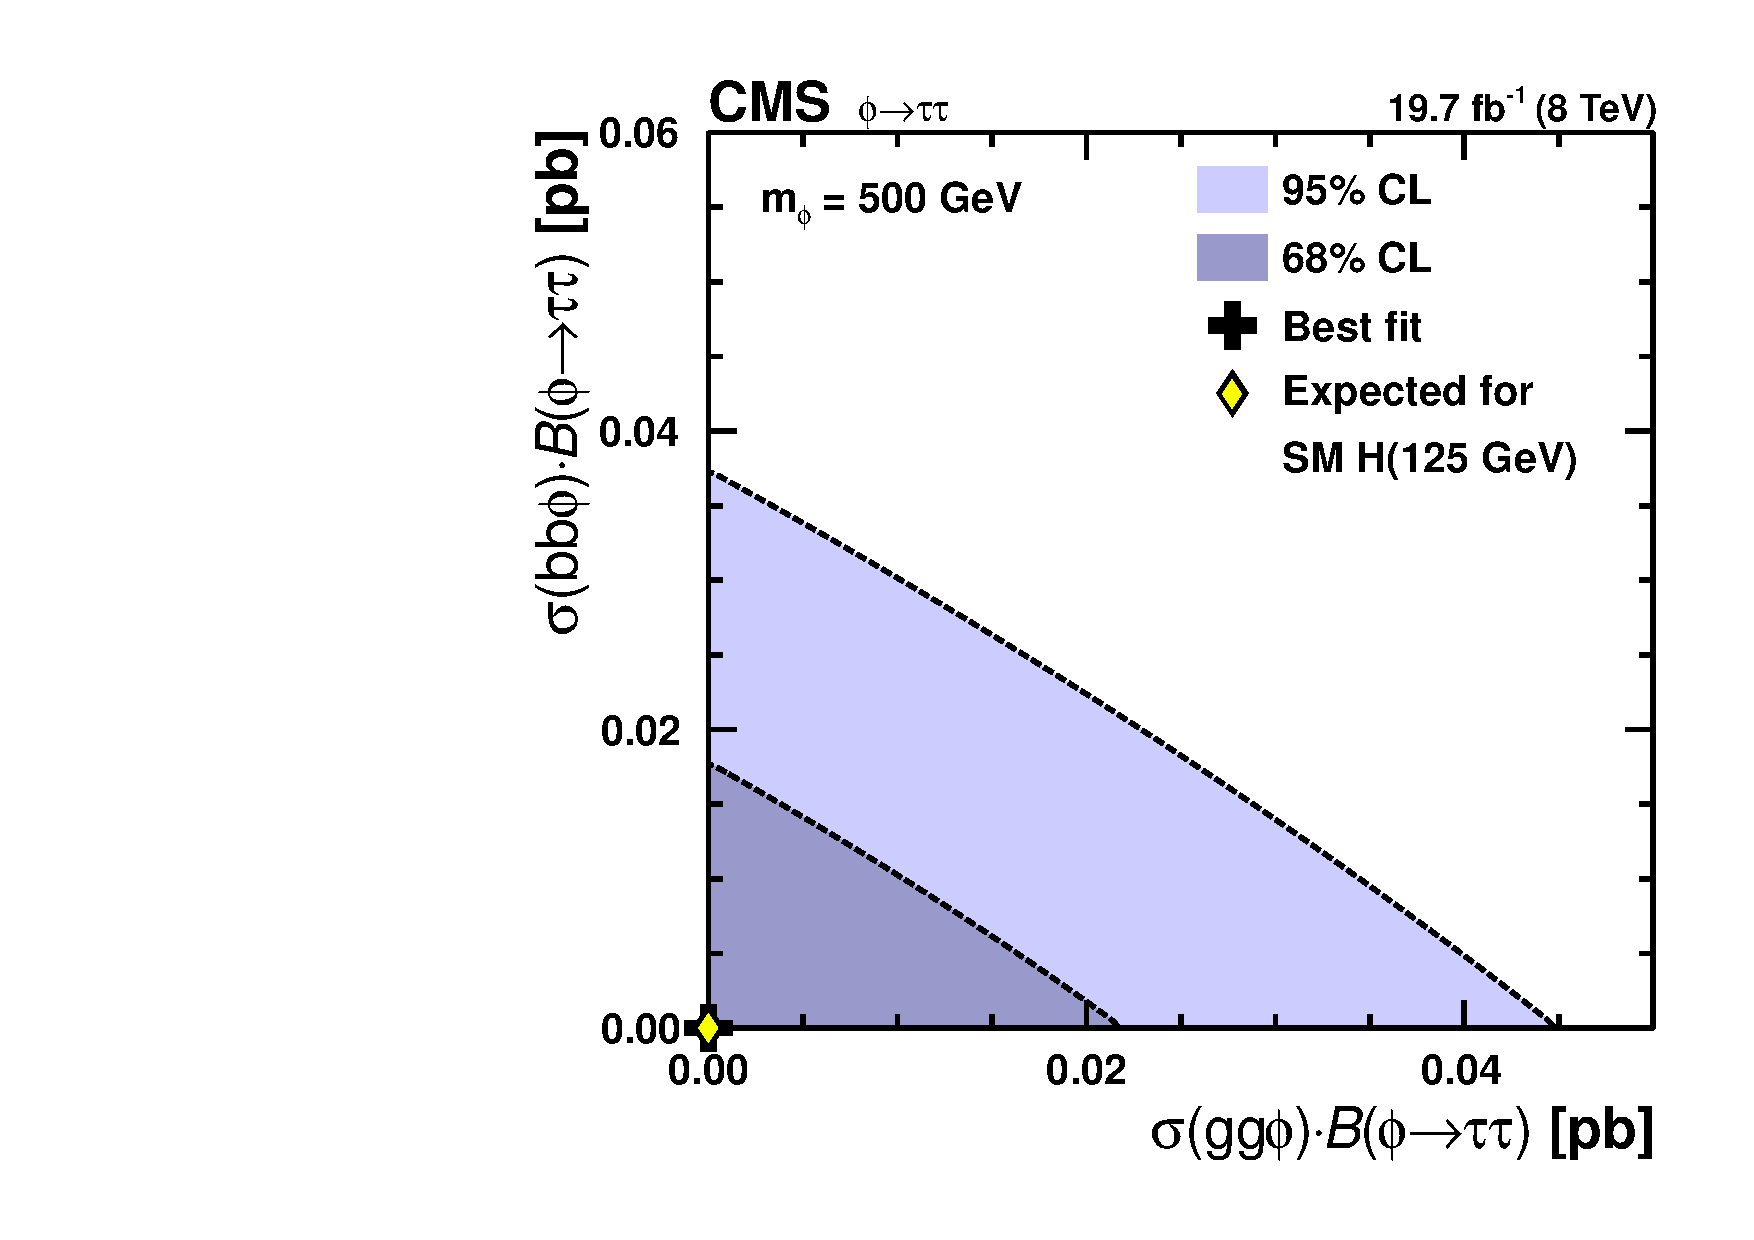
\includegraphics[width=0.5\textwidth]{plots/htt-mssm/bbb-ggH-bbH-scan-GGH-BBH-500.pdf}}
\subfloat[]{
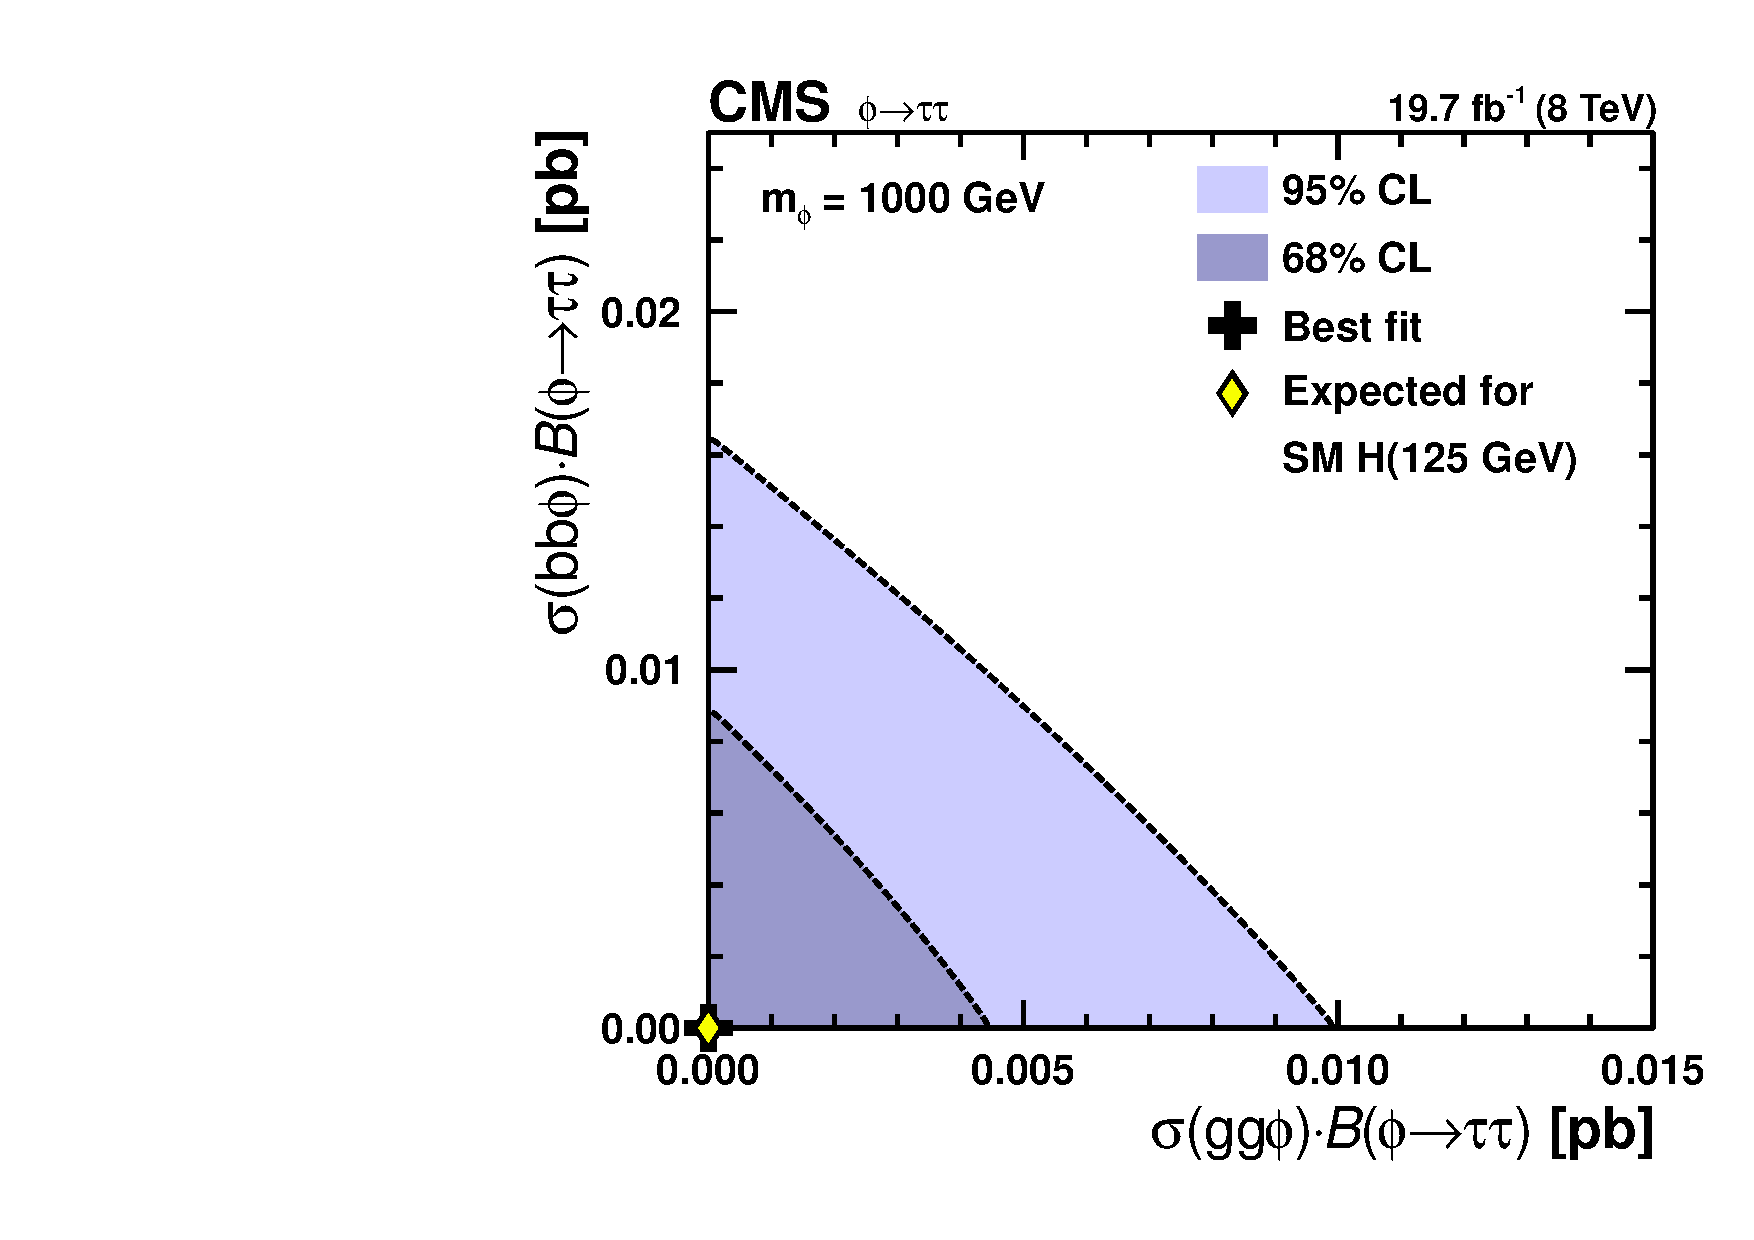
\includegraphics[width=0.5\textwidth]{plots/htt-mssm/bbb-ggH-bbH-scan-GGH-BBH-1000.pdf}}
\caption[2-D likelihood scans showing the best fit values for the cross-section
times branching ratio of the gluon fusion (x-axis) and b-associated production
(y-axis) processes using $8\,\TeV$ data.]{2-D likelihood scans showing the best fit values for the cross-section
times branching ratio of the gluon fusion (x-axis) and b-associated production
(y-axis) processes using $8\,\TeV$ data. Shown for $m_{\Pphi}$ values of
$125\,\GeV$ (a), $300\,\GeV$ (b), $500\,\GeV$ (c) and
$1\,\TeV$ (d). The best fit point is indicated along with the best fit
point which would be obtained if there was a $125\,\GeV$ \ac{SM} Higgs boson in the data \cite{HIG-13-021}.}
\label{fig:2Dlikelihood}
\end{figure}

\subsubsection{Limits on $\sigma \times \cal{B}$}

The simplest type of limit produced in the \ac{MSSM} analysis is analogous to the 
expected limit on $\mu$ produced in the \ac{SM} analysis (figure
\ref{fig:results-limit}). In the \ac{MSSM} analysis, instead of setting a limit
on the signal strength modifier with reference to a benchmark cross-section, a
more model-independent limit is given on cross-section times branching ratio
for the Higgs production process. This can then be interpreted in many different
benchmark models. A limit is set separately for each of the two dominant production modes,
$\Pqb\Pqb\Pphi$ and $\Pg\Pg\Pphi$, again in a `single
resonance' search for $\Pphi$. It is not possible to
completely disentangle the two production modes - as shown in
section~\ref{sec:mssmEventSelection} the categorisation does not completely
separate the signal contributions, and some $\Pqb\Pqb\Pphi$ signal is
found in no b--tag category and some $\Pg\Pg\Phi$ in the b--tag category. Hence
to produce a limit on each process separately, the other signal process is
`profiled'. This means that it is allowed to float in the fit in a similar way
to one of the nuisance parameters. 

Figure \ref{fig:mssmModelIndependent} shows the expected and observed limit on
cross-section times branching ratio for the $\Pg\Pg\Pphi$ and $\Pqb\Pqb\Pphi$
production processes. The expected limit and the corresponding 1 and 2$\sigma$ bands
are generated in the same way as in figure \ref{fig:results-limit} b), by
running toys with an \ac{SM} Higgs injected.
In this way the observed limit is compared to an expected including both the
backgrounds and an \ac{SM} Higgs. 

\begin{figure}[tbh]
\subfloat[]{
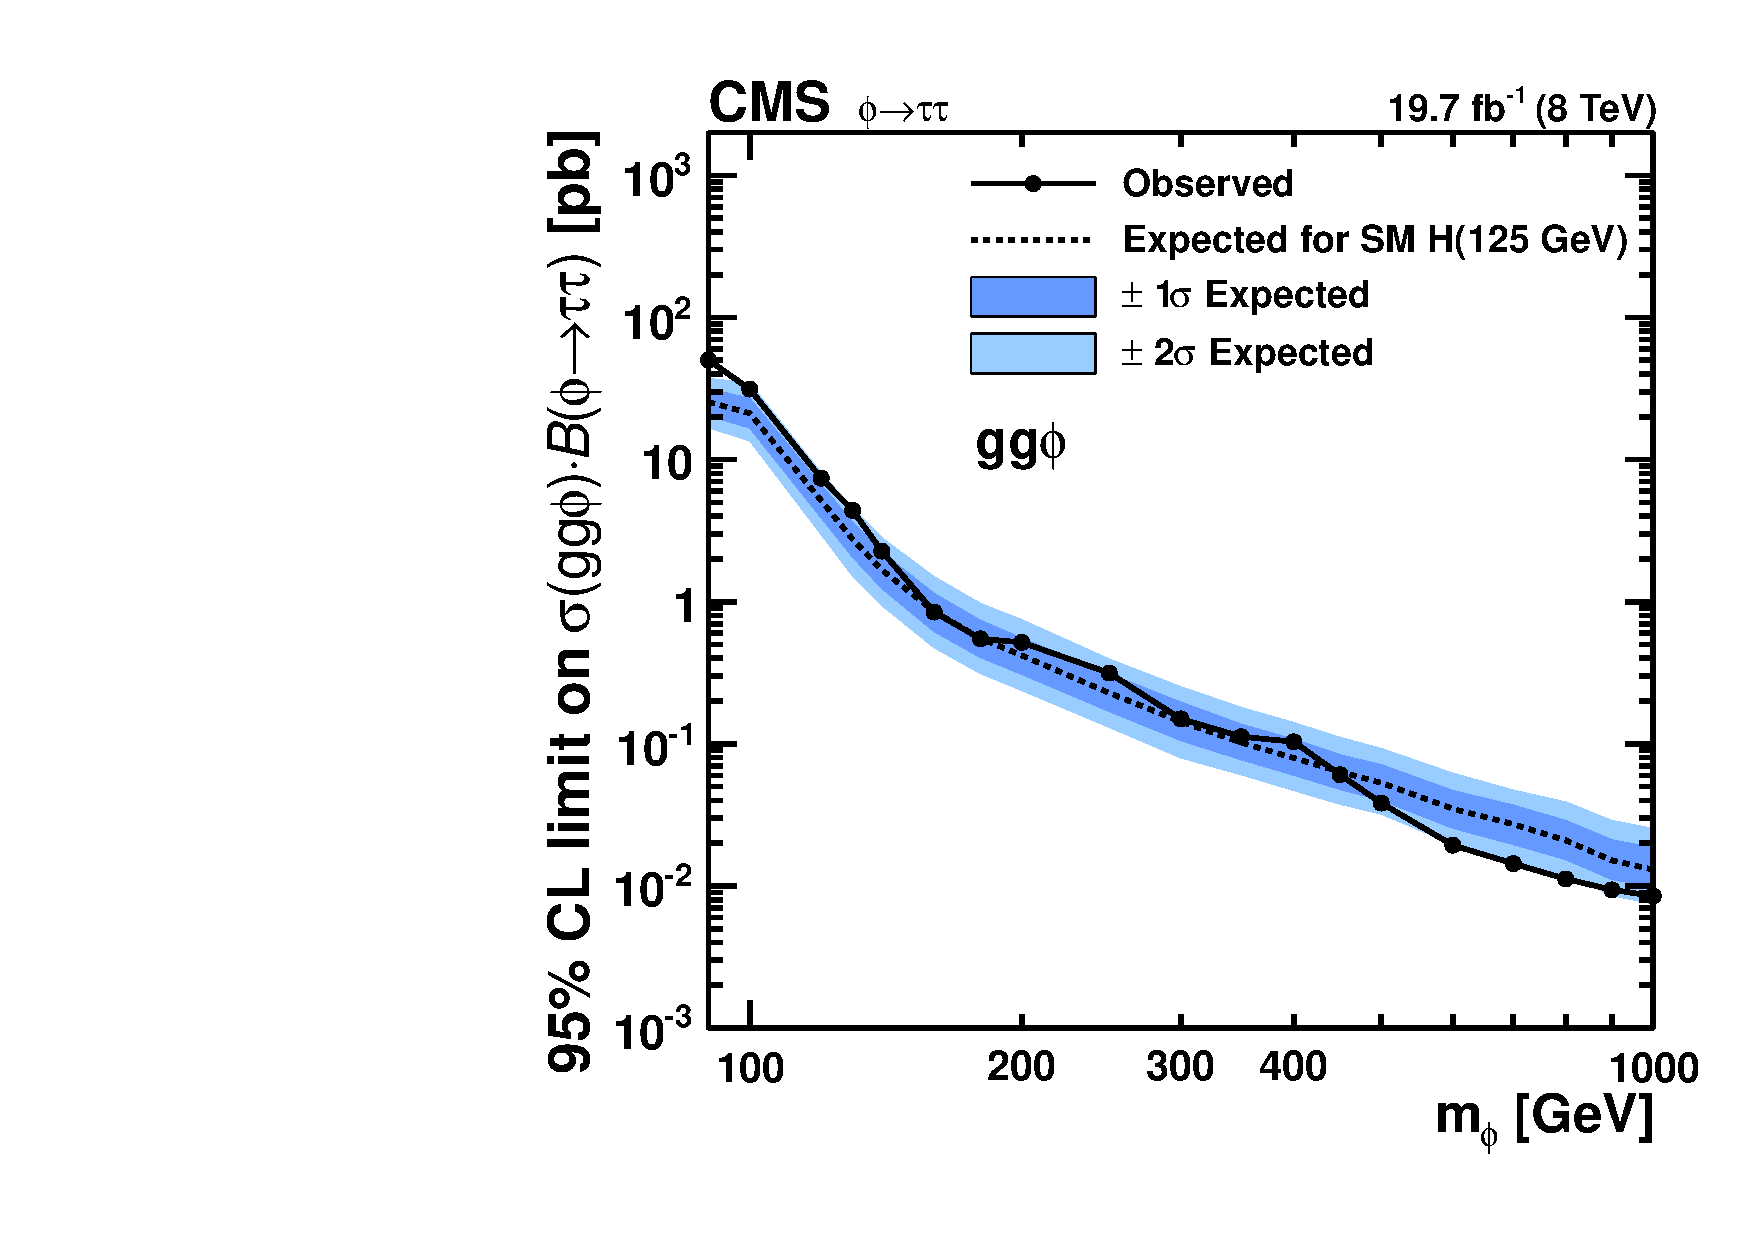
\includegraphics[width=0.5\textwidth]{plots/htt-mssm/cmb_ggH-limit.pdf}}
\subfloat[]{
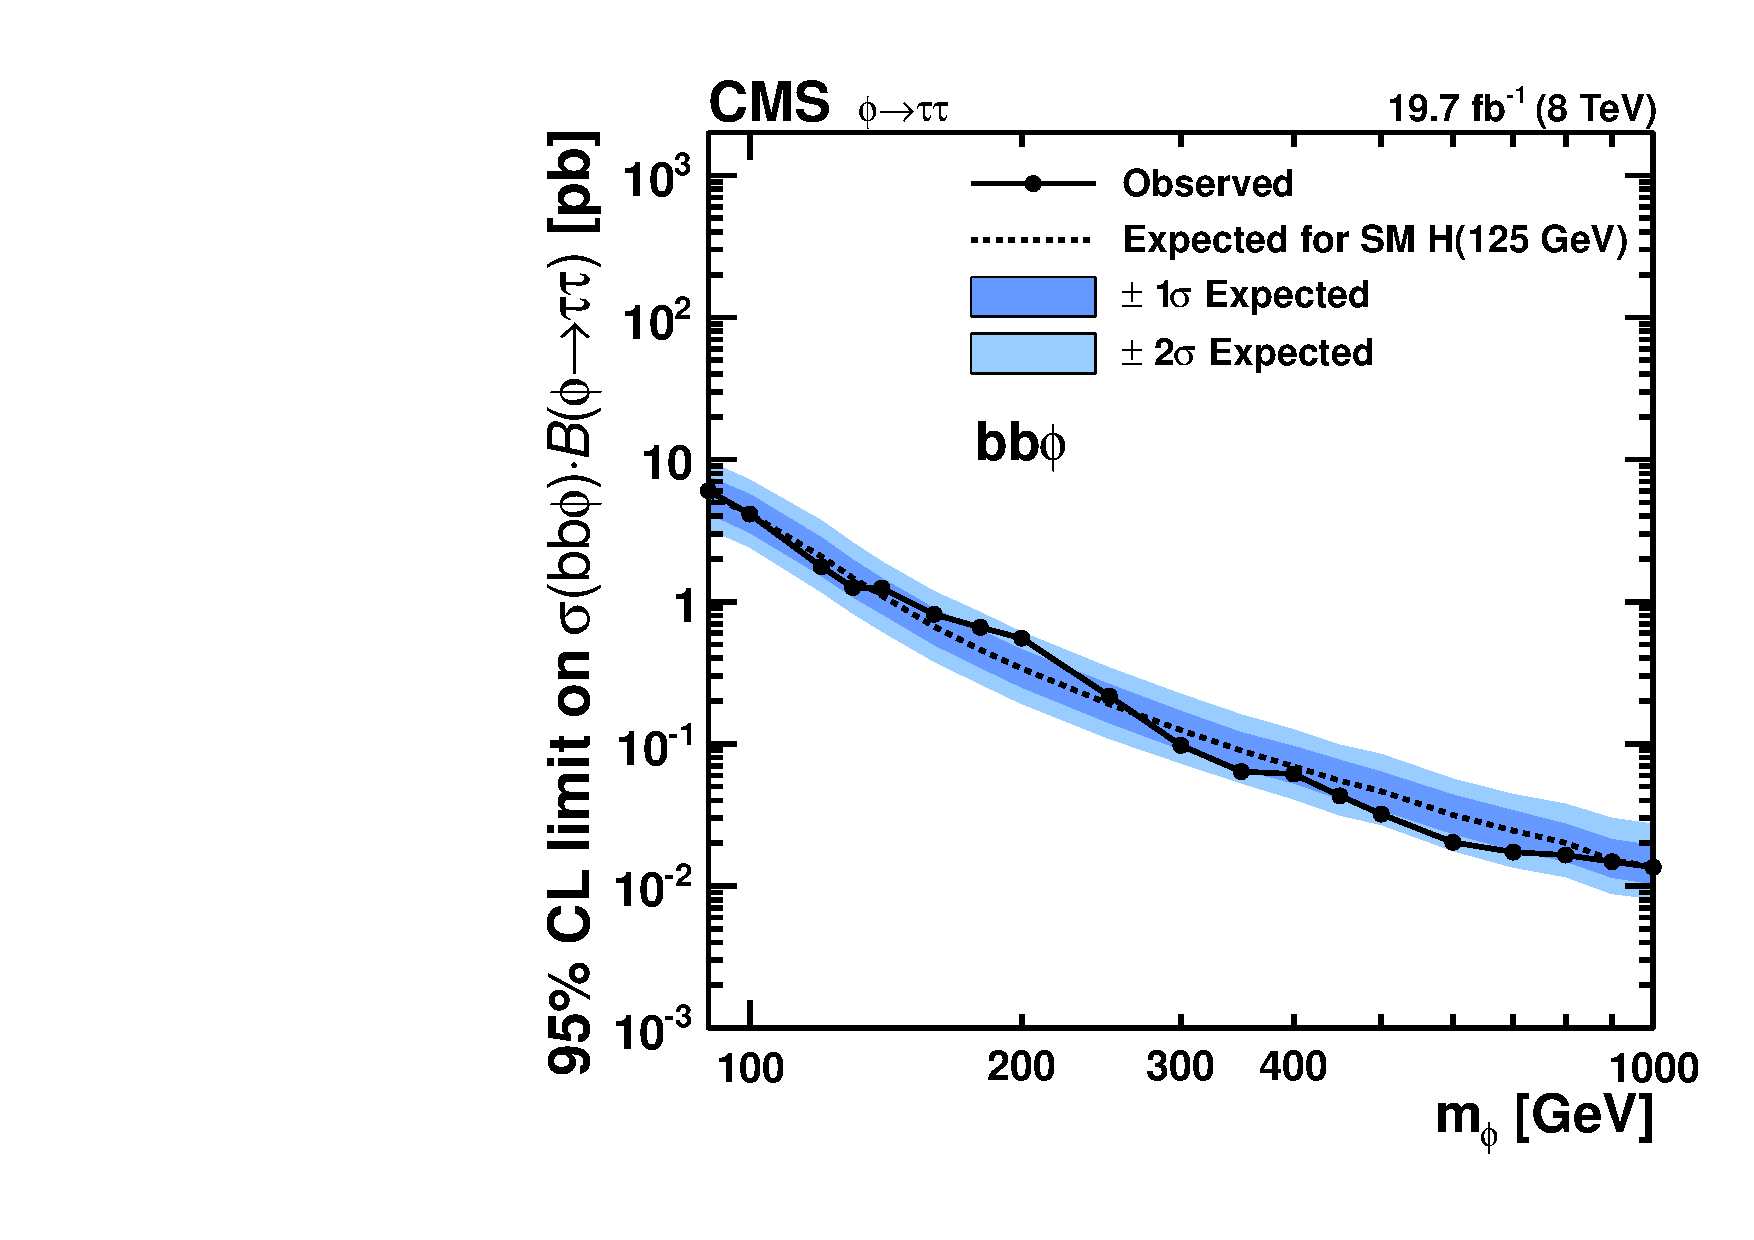
\includegraphics[width=0.5\textwidth]{plots/htt-mssm/cmb_bbH-limit.pdf}}
\caption[Limits on cross-section times branching ratio for a) gluon fusion Higgs
production and b) b-associated Higgs production for the combination of all
channels and categories in the $8\,\TeV$ data.]{Limits on cross-section times branching ratio for a) gluon fusion Higgs
production and b) b-associated Higgs production for the combination of all
channels and categories in the $8\,\TeV$ data. For each limit the other production process is
profiled. The observed limit is compared with an expected limit which includes
the \ac{SM} Higgs \cite{HIG-13-021}.}
\label{fig:mssmModelIndependent}
\end{figure}

The reason for comparing the observed with an expected including the \ac{SM}
Higgs, both here and in the 2D likelihood results, 
is that the results cannot be interpreted in the context of the \ac{MSSM} without taking into account
the fact that there is $3\sigma$ evidence of an \ac{SM}-like Higgs boson decaying
into taus. Despite the fact that the categorisation of events is chosen to
enhance selection of a \ac{MSSM} signal rather than a \ac{SM} signal, the
selection is still very close to that of the \ac{SM} analysis and hence there is
still some sensitivity to the \ac{SM} Higgs in the \ac{MSSM} analysis. Thus any
excess in data over background must be interpreted very carefully, since it
does not automatically mean evidence of an \ac{MSSM} signal when it could be
from the \ac{SM} Higgs. 

\subsection{Model dependent results}
\label{sec:modeldependent}

The model independent results described in the previous section are open to
interpretation in a variety of models. It is also interesting to look more
closely at the interpretation of the results in particular benchmark scenarios.
Such results are referred to as `model-dependent'. Model-dependent searches are
conducted in a plane of the two free parameters in the model, usually $m_{\PA}$
and $\tan\beta$. At each point in the phase space, the cross-section times
branching ratio for each of the three neutral Higgs bosons is calculated, taking
into account both production processes. The contributions of the three Higgs
bosons are then combined into one template for the final fit. Hence, unlike in the
model-independent `single resonance' searches, the consistency of the data with
all three Higgs bosons is considered. 

The sensitivity to the \ac{SM} Higgs becomes even more important in a
model-dependent result. As discussed in
section~\ref{sec:mssmbenchmarks}, the \ac{MSSM} benchmark scenarios being tested in this
analysis are required to be consistent with experimental measurements of the
$125\,\GeV$ Higgs bosons. Hence in such scenarios, one of the three neutral Higgs
bosons must be very similar to the \ac{SM} $125\,\GeV$ Higgs boson. This means
that by construction an \ac{MSSM} signal from one of these benchmarks looks a
lot like the \ac{SM} signal, with the exception of the requirement of the
additional two Higgs bosons.

Hence when interpreting the results of the \ac{MSSM} search in the context of an
\ac{MSSM} benchmark scenario, it is not enough to simply construct a limit from
considering the background-only hypothesis compared with the
signal-plus-background hypothesis. Instead, a limit is built based on
whether the data agrees better than the background plus \ac{SM} signal or
background plus \ac{MSSM} signal hypothesis.

\subsubsection{MSSM and SM hypothesis testing}

To compare two different signal hypotheses, the likelihood function as described
in equation~\ref{eq:LikelihoodFunction} must be modified. This likelihood compares 
the observed data with an expected constructed as
$\mu \cdot s(\theta) + b(\theta)$. This must be modified to compare the data with the
following:
\begin{equation}
\mathcal{L}(\text{data} | \mu \cdot s(\theta) + b(\theta)) \rightarrow
\mathcal{L}(\text{data} | M(\mu,\theta)),
\end{equation}
with
\begin{equation}
M(\mu,\theta) = \mu \cdot s_{\text{MSSM}}(\theta) + (1-\mu) \cdot
s_{\text{SM}}(\theta) + b(\theta), 
\end{equation}

where $s_{\text{MSSM}}(\theta)$ and $s_{\text{SM}}(\theta)$ are the
signal expectations in the \ac{MSSM} and \ac{SM} hypotheses respectively. In
this likelihood the signal strength modifier $\mu$ connects both expectations,
with the null hypothesis being the \ac{SM} for $\mu=0$ and the alternative
hypothesis the \ac{MSSM} for $\mu=1$. This choice ensures that the model does
not allow for the coexistence of the \ac{SM} and \ac{MSSM} hypotheses. 

With this likelihood, a slightly different form of the test statistic must be
built compared with that of equation~\ref{eq:ProfileLikelihood}. In the test
statistic used at the LHC, the numerator is defined for some signal
strength $\mu$ compared with the signal strength which maximises the likelihood,
$\hat{\mu}$. Here is required instead a version of the test statistic which tests
two fixed values of $\mu$ against on another. For this a test statistic
which was used at the Tevatron, and hence is referred to as the ``TEV'' test
statistic, is used, which takes the general form:

\begin{equation}
%q_{0} = -2\ln ( \frac{\mathcal{L}(\text{data}|\mu\cdot s(\hat{\theta_{\mu}}) + b(\hat{\theta_{\mu}})) }
%{\mathcal{L}(\text{data}|b(\hat{\theta_{0}}))} )
q_{0} = -2\ln\frac{\mathcal{L}(\text{data}| \mu,\hat{\theta_{\mu}} ) }
{\mathcal{L}(\text{data}|\mu=0,\hat{\theta_{0}})}
\;\; \text{with the constraint} \; 0\leq\mu\, .
\end{equation}

In this test statistic a numerator corresponding to the signal strength $\mu$ is
compared with a denominator corresponding to $\mu=0$. Hence the required form of this
test statistic corresponds to the comparison between
$\mu=1$ and $\mu=0$, hence:

\begin{equation}
q_{\text{MSSMvsSM}} = -2\ln\frac{\mathcal{L}(\text{data}| M(1,\hat{\theta_{1}}) ) }
{\mathcal{L}(\text{data}| M(0,\hat{\theta_{0}}) )}.
\label{eq:qMSSMvsSM}
\end{equation}

The disadvantage of a test statistic of this type is that there is no asymptotic
approximation, and so the distributions of the probability distribution
functions for the test statistic must be generated using toys. Figure
\ref{fig:toydistribution} shows the distributions obtained using toys with
either the \ac{SM} or \ac{MSSM} signal hypothesis, and the observed value of the
test statistic is shown. For this example $m_{\PA}-\tan\beta$ point, it can be
seen that the separation between the two distributions is good, and hence this
point is able to be excluded in the absence of an excess. It can be seen that
the observed agrees better with the \ac{SM} hypothesis than the \ac{MSSM}
hypothesis, indicating the lack of such an excess over the expectation from
backgrounds plus \ac{SM} Higgs. 

\begin{figure}[tbh]
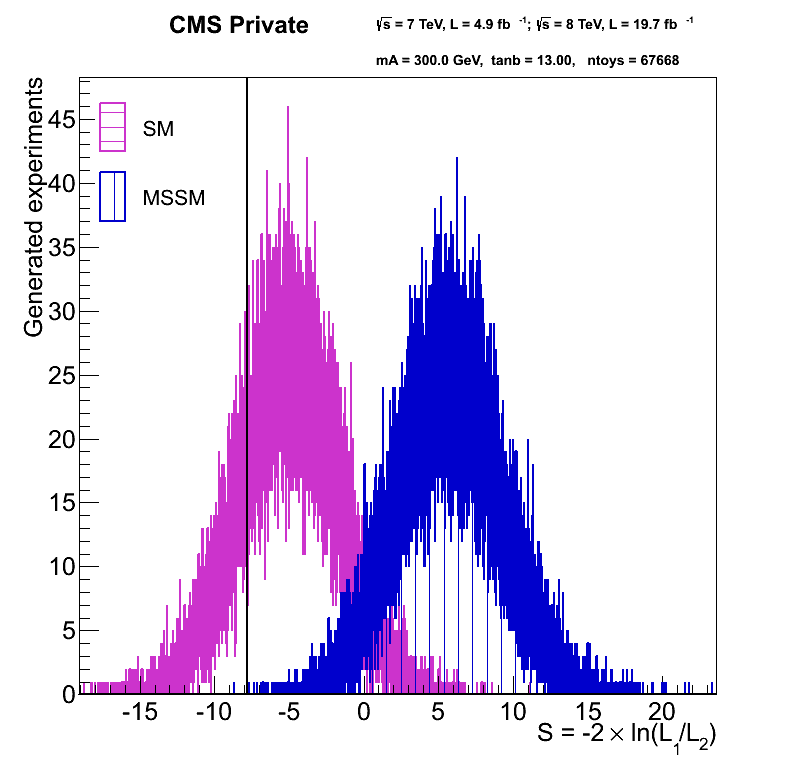
\includegraphics[width=0.7\textwidth]{plots/htt-mssm/sigsep_13.png}
\caption[Distributions of the test statistic for toys with SM or MSSM
signal injected for $m_{\PA} = 300\,\GeV$, $\tan\beta = 13$ in the $m_{h}^{\text{max}}$
scenario.]{Distributions of the test statistic for toys with \ac{SM} or
\ac{MSSM} signal injected for $m_{\PA} = 300\,\GeV$, $\tan\beta = 13$ in the $m_{h}^{\text{max}}$
scenario. The black vertical line indicates the observed value of the test
statistic. The separation of the distributions is such that this point can be
excluded at 95$\%$ CL}
\label{fig:toydistribution}
\end{figure}

The $\mathrm{CL_{s}}$ values are obtained using these probability distributions as
follows:

\begin{equation}
A = \int_{q_{0}^{x}}^{\infty}f(q_{0},\hat{\theta}_{0})\mathrm{d}q_{0}\, \\
B = \int_{q_{1}^{x}}^{\infty}f(q_{1},\hat{\theta}_{1})\mathrm{d}q_{1}\, \\
\mathrm{CL_{s}} = \frac{B}{A},
\end{equation}

where $x$ is either the 0.025, 0.16, 0.5, 0.84 or 0.975 quantile of the SM
probability density function (corresponding to -2$\sigma$, -1$\sigma$, expected,
$+1\sigma$, $+2\sigma$ exclusion) or the observed value. To obtain the final limit, 
a scan is performed in the two parameter plane and
the $\mathrm{CL_{s}}$ is calculated at each point in a 2D grid. Each point is excluded at
95$\%$ CL if $\mathrm{CL_{s}}<0.05$. A contour is drawn to connect the excluded points
using interpolation between neighbouring points in the grid.

Figure \ref{fig:hypotestcompare} shows the comparison between the exclusion
limits obtained using the conventional method of comparing \ac{MSSM} signal
hypothesis against background-only with the asymptotic approximation 
and using this new method to compare the
\ac{MSSM} and \ac{SM} hypotheses for the example of the $m_{\Ph}^\text{max}$
scenario. The left hand plot includes a line which shows
the effect of injecting an \ac{SM} signal into this limit. It can clearly be
seen that the effect of a possible \ac{SM} Higgs is not negligible and that a
possible difference between observed and expected limit in these plots could be 
the result of the \ac{SM} Higgs in the dataset. In these results the data are 
consistent with both the background only and the background plus \ac{SM} signal hypotheses.

\begin{figure}[tbh]
\subfloat[]{
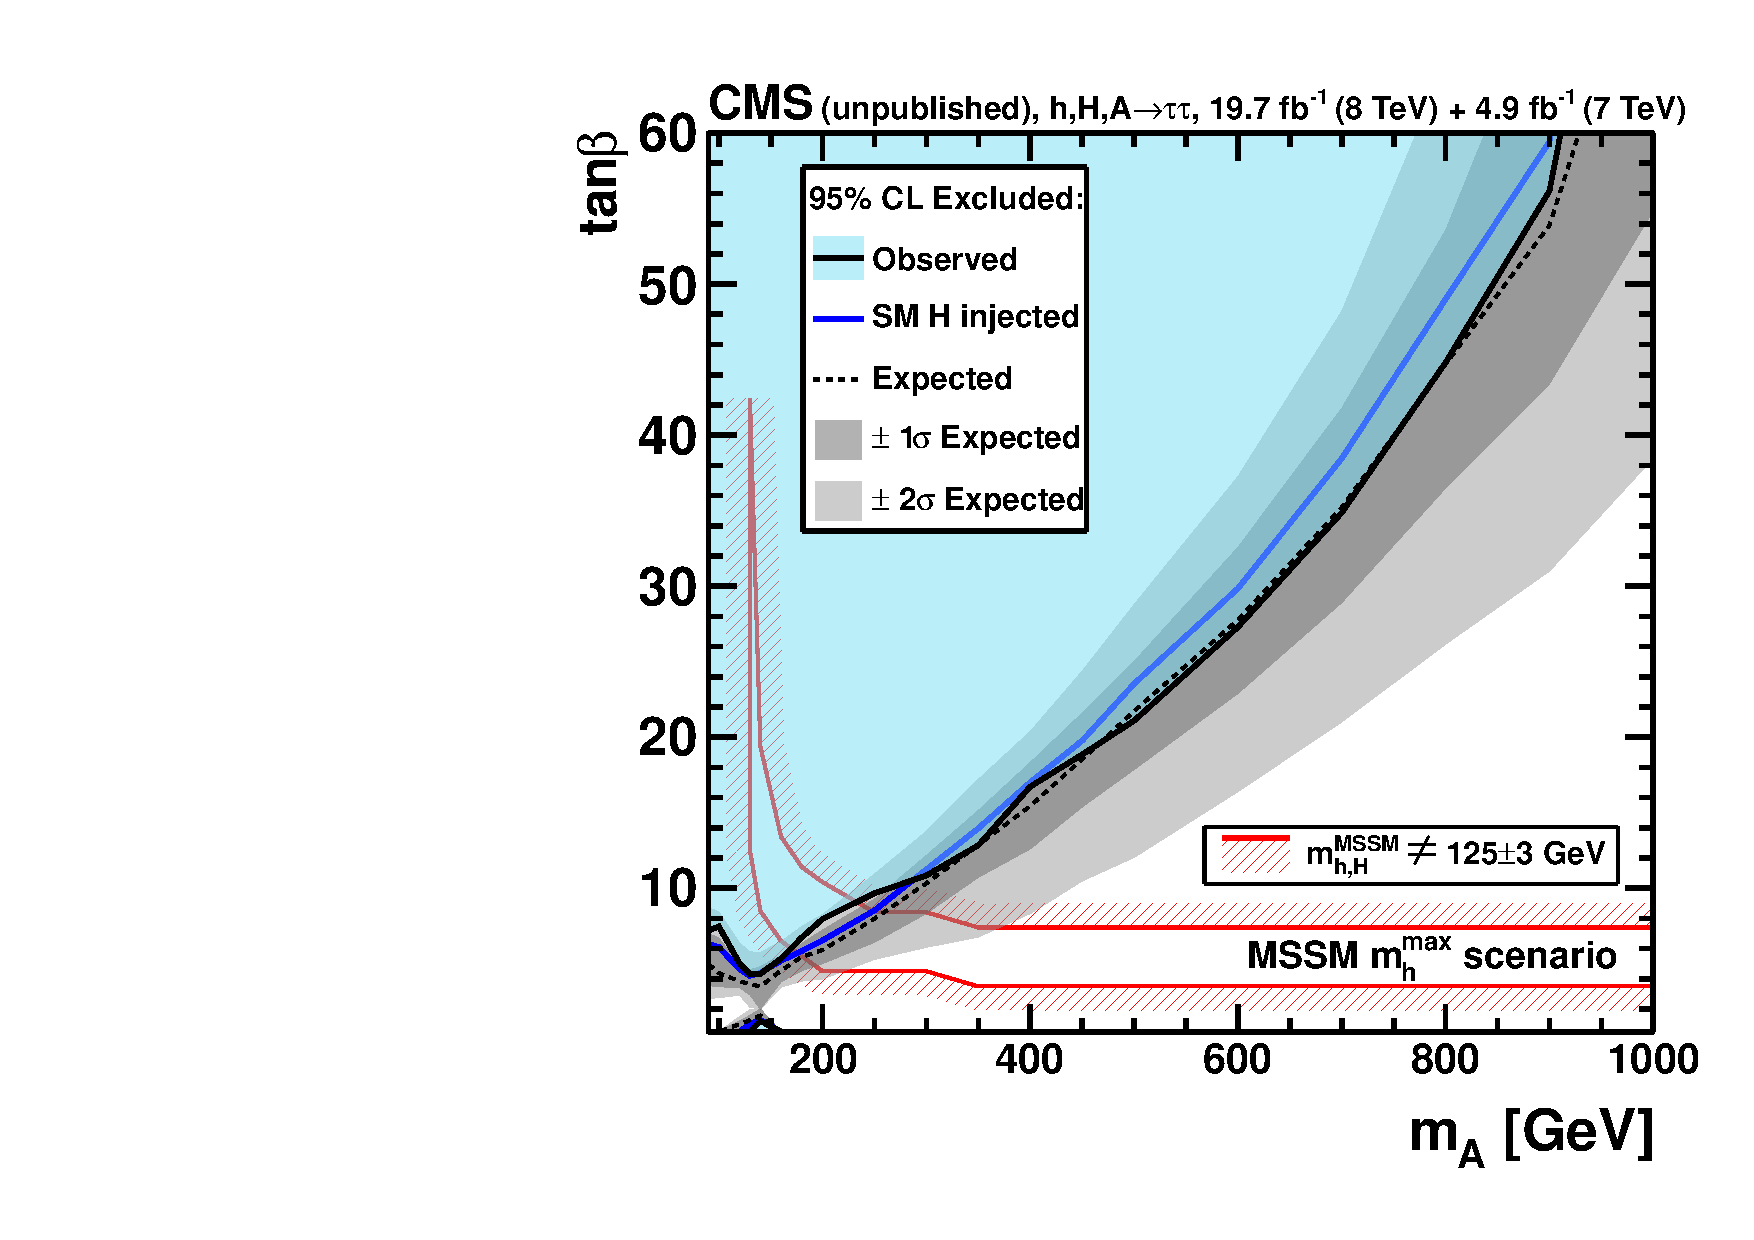
\includegraphics[width=0.5\textwidth]{plots/htt-mssm/cmb_mhmax-mA-tanb-SMinjected.pdf}}
\subfloat[]{
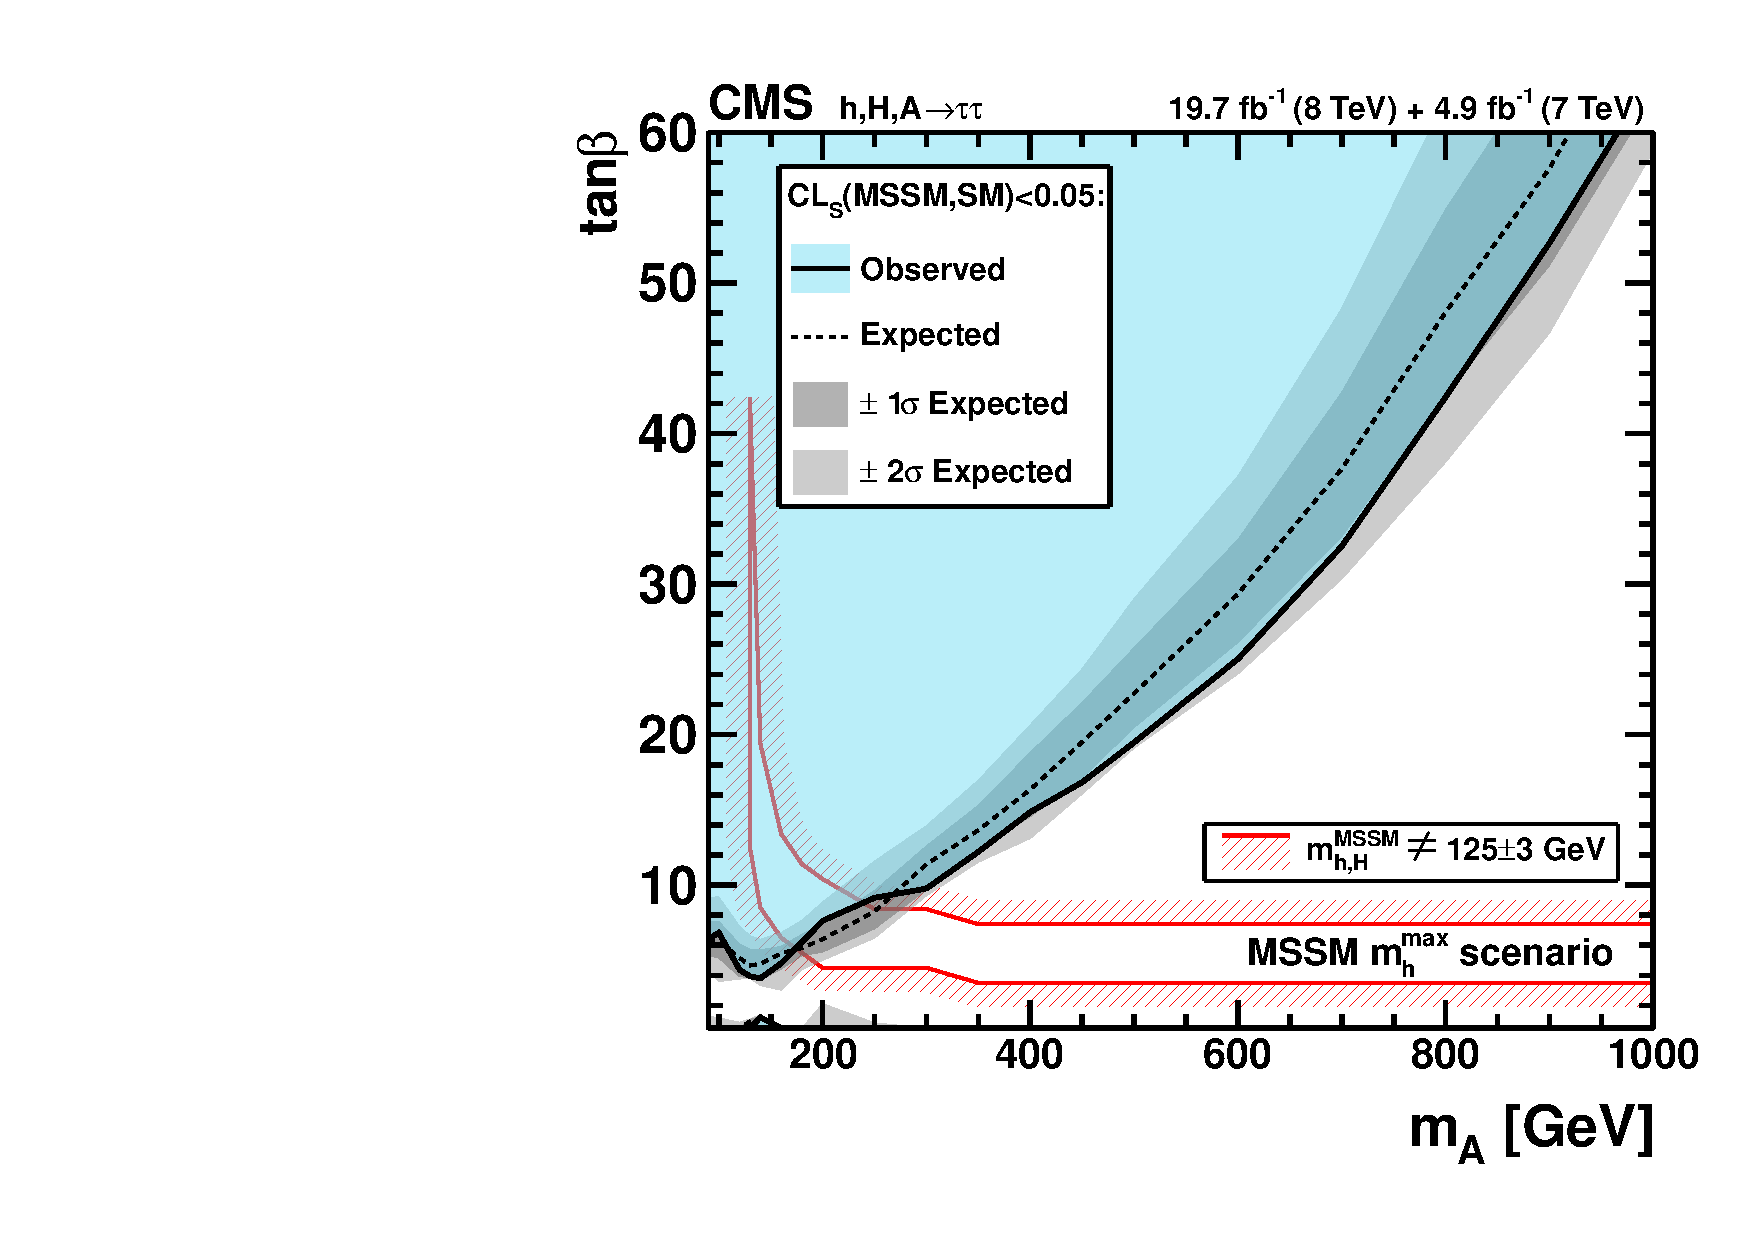
\includegraphics[width=0.5\textwidth]{plots/htt-mssm/cmbRL_mhmax-HypoTest.pdf}}
\caption[Expected and observed limit in the $m_{\PA}-\tan\beta$ plane of the
$m_H^{\text{max}}$ scenario.]{Expected and observed limit in the $m_{\PA}-\tan\beta$ plane of the
$m_H^{\text{max}}$ scenario. In the left hand plot, the \ac{MSSM} signal is
compared with the background only hypothesis. In the right hand plot, hypothesis
separation testing compares the \ac{MSSM} hypothesis with the \ac{SM}
hypothesis. The red area indicates the region of phase space which is already
excluded by the Higgs mass constraint of $125\pm3\,\GeV$ \cite{HIG-13-021-twiki,HIG-13-021}.}
\label{fig:hypotestcompare}
\end{figure}


Note that the red areas indicated in figure \ref{fig:hypotestcompare} show the
region of phase space which is already ruled out by the constraint on the Higgs
mass being close to $125\,\GeV$, with a $\pm 3\,\GeV$ uncertainty due to
theoretical calculations in the \ac{MSSM}. The $m_{\Ph}^{\text{max}}$ scenario
is almost entirely ruled out by this constraint, as discussed in
section~\ref{sec:mssmbenchmarks}. Figures \ref{fig:mhmodpmhmodm} to \ref{fig:tauphobiclowmH}
show the result interpreted in newer scenarios which better incorporate a
$125\,\GeV$ Higgs. Large areas of the phase space in these scenarios is ruled out
by the lack of an excess in this analysis.


\begin{figure}[tbh]
\subfloat[]{
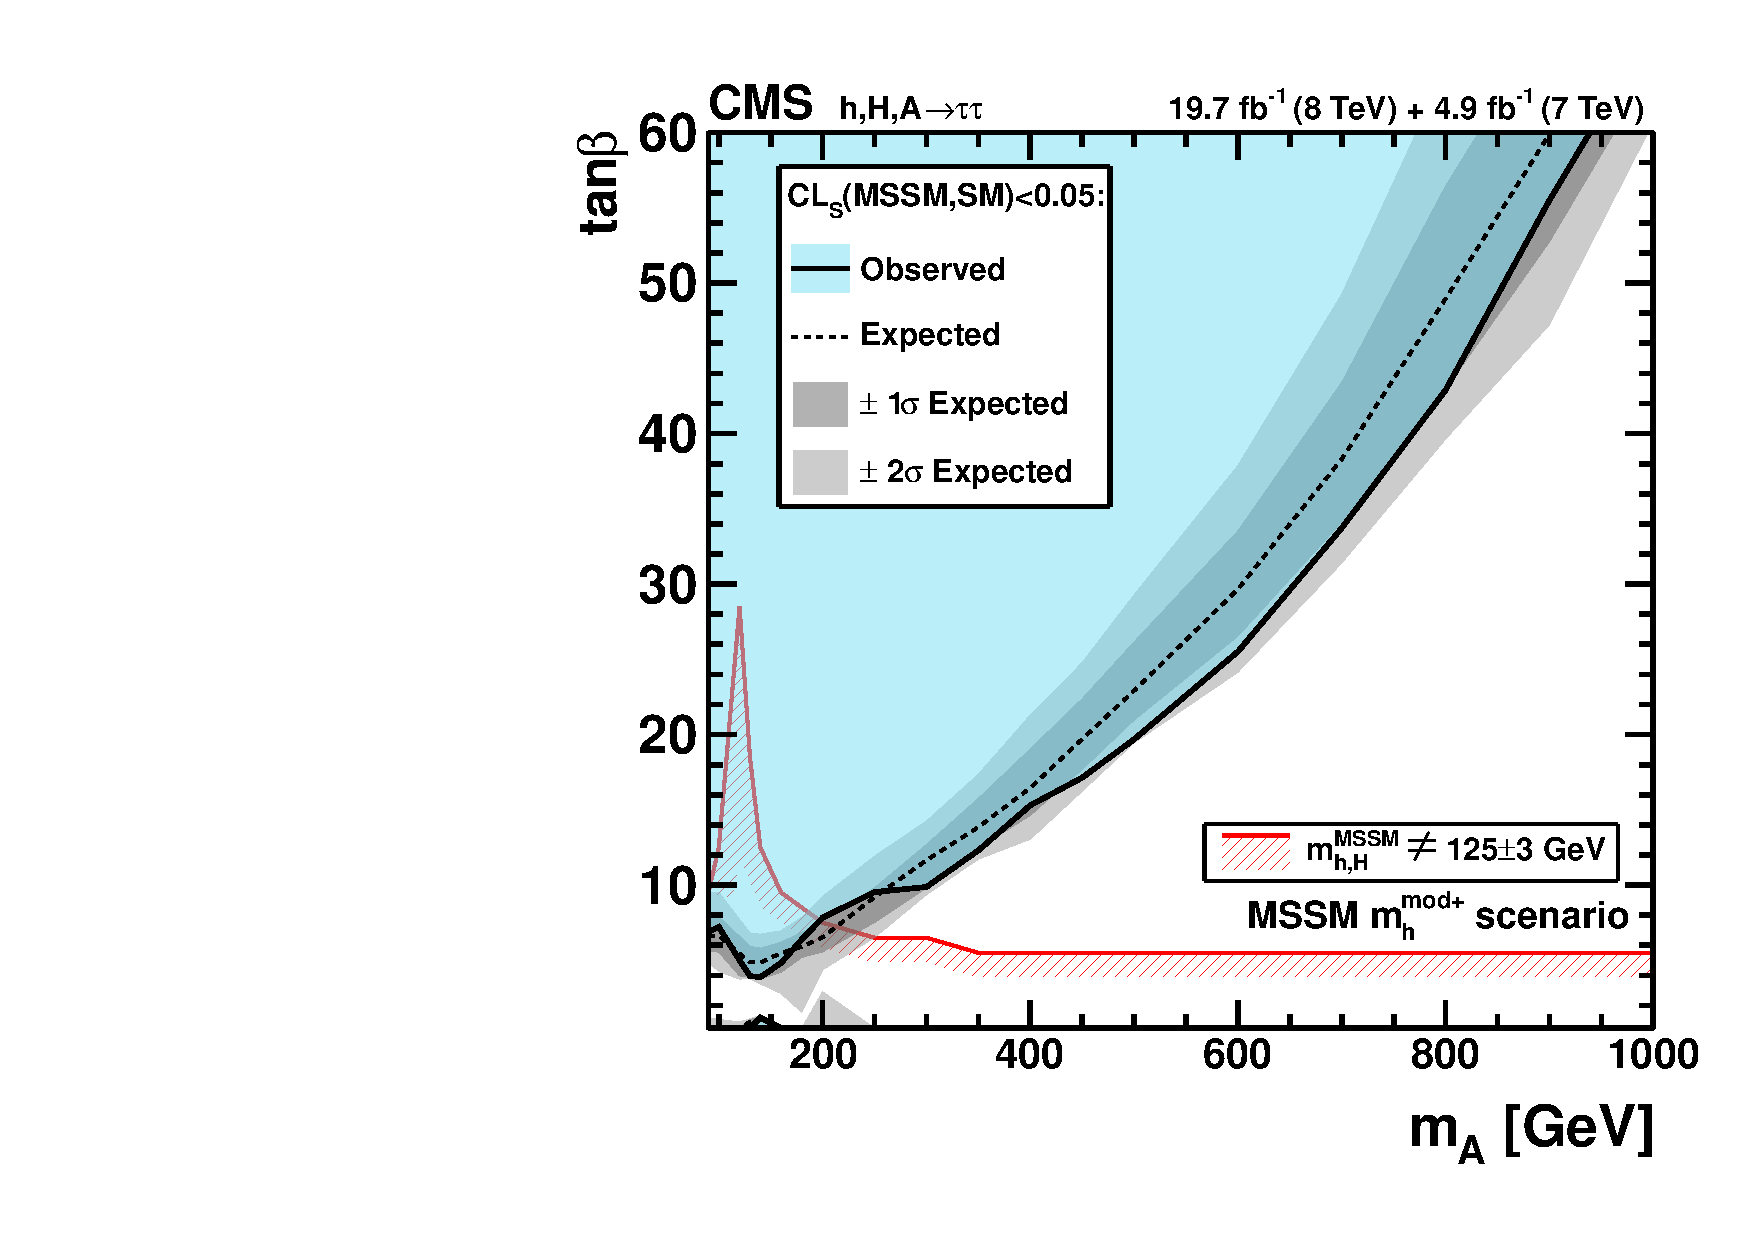
\includegraphics[width=0.5\textwidth]{plots/htt-mssm/cmbRL_mhmodp-HypoTest.pdf}}
\subfloat[]{
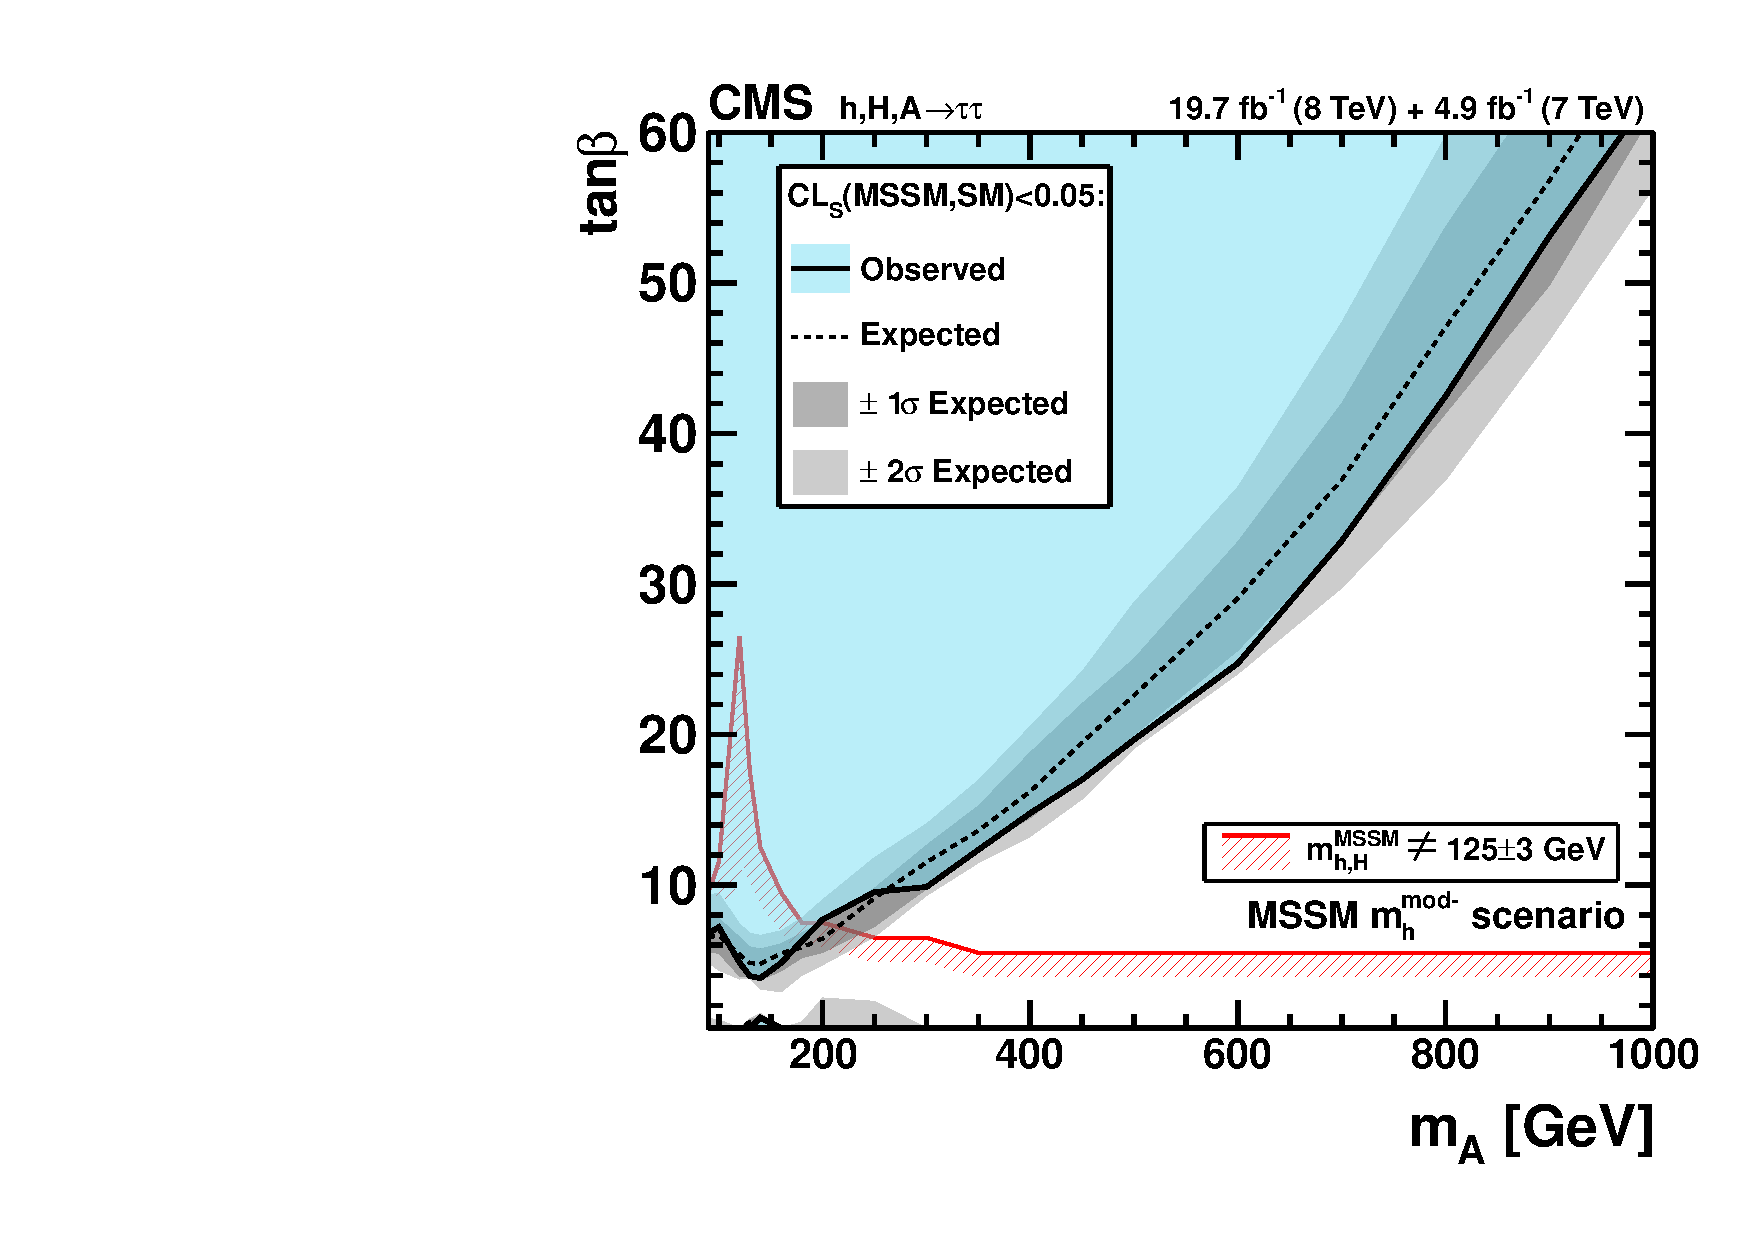
\includegraphics[width=0.5\textwidth]{plots/htt-mssm/cmbRL_mhmodm-HypoTest.pdf}}
\caption[Expected and observed limit in the $m_{\PA}-\tan\beta$ plane of the
$m_H^{\text{mod+}}$ scenario (a) and $m_H^{\text{mod-}}$ scenario (b).]
{Expected and observed limit in the $m_{\PA}-\tan\beta$ plane of the
$m_H^{\text{mod+}}$ scenario (a) and $m_H^{\text{mod-}}$ scenario (b). Hypothesis
separation testing is used to compare the \ac{MSSM} hypothesis with the \ac{SM}
hypothesis. The red area indicates the region of phase space which is already
excluded by the Higgs mass constraint of $125\pm3\,\GeV$ \cite{HIG-13-021}.}
\label{fig:mhmodpmhmodm}
\end{figure}

\begin{figure}[tbh]
\subfloat[]{
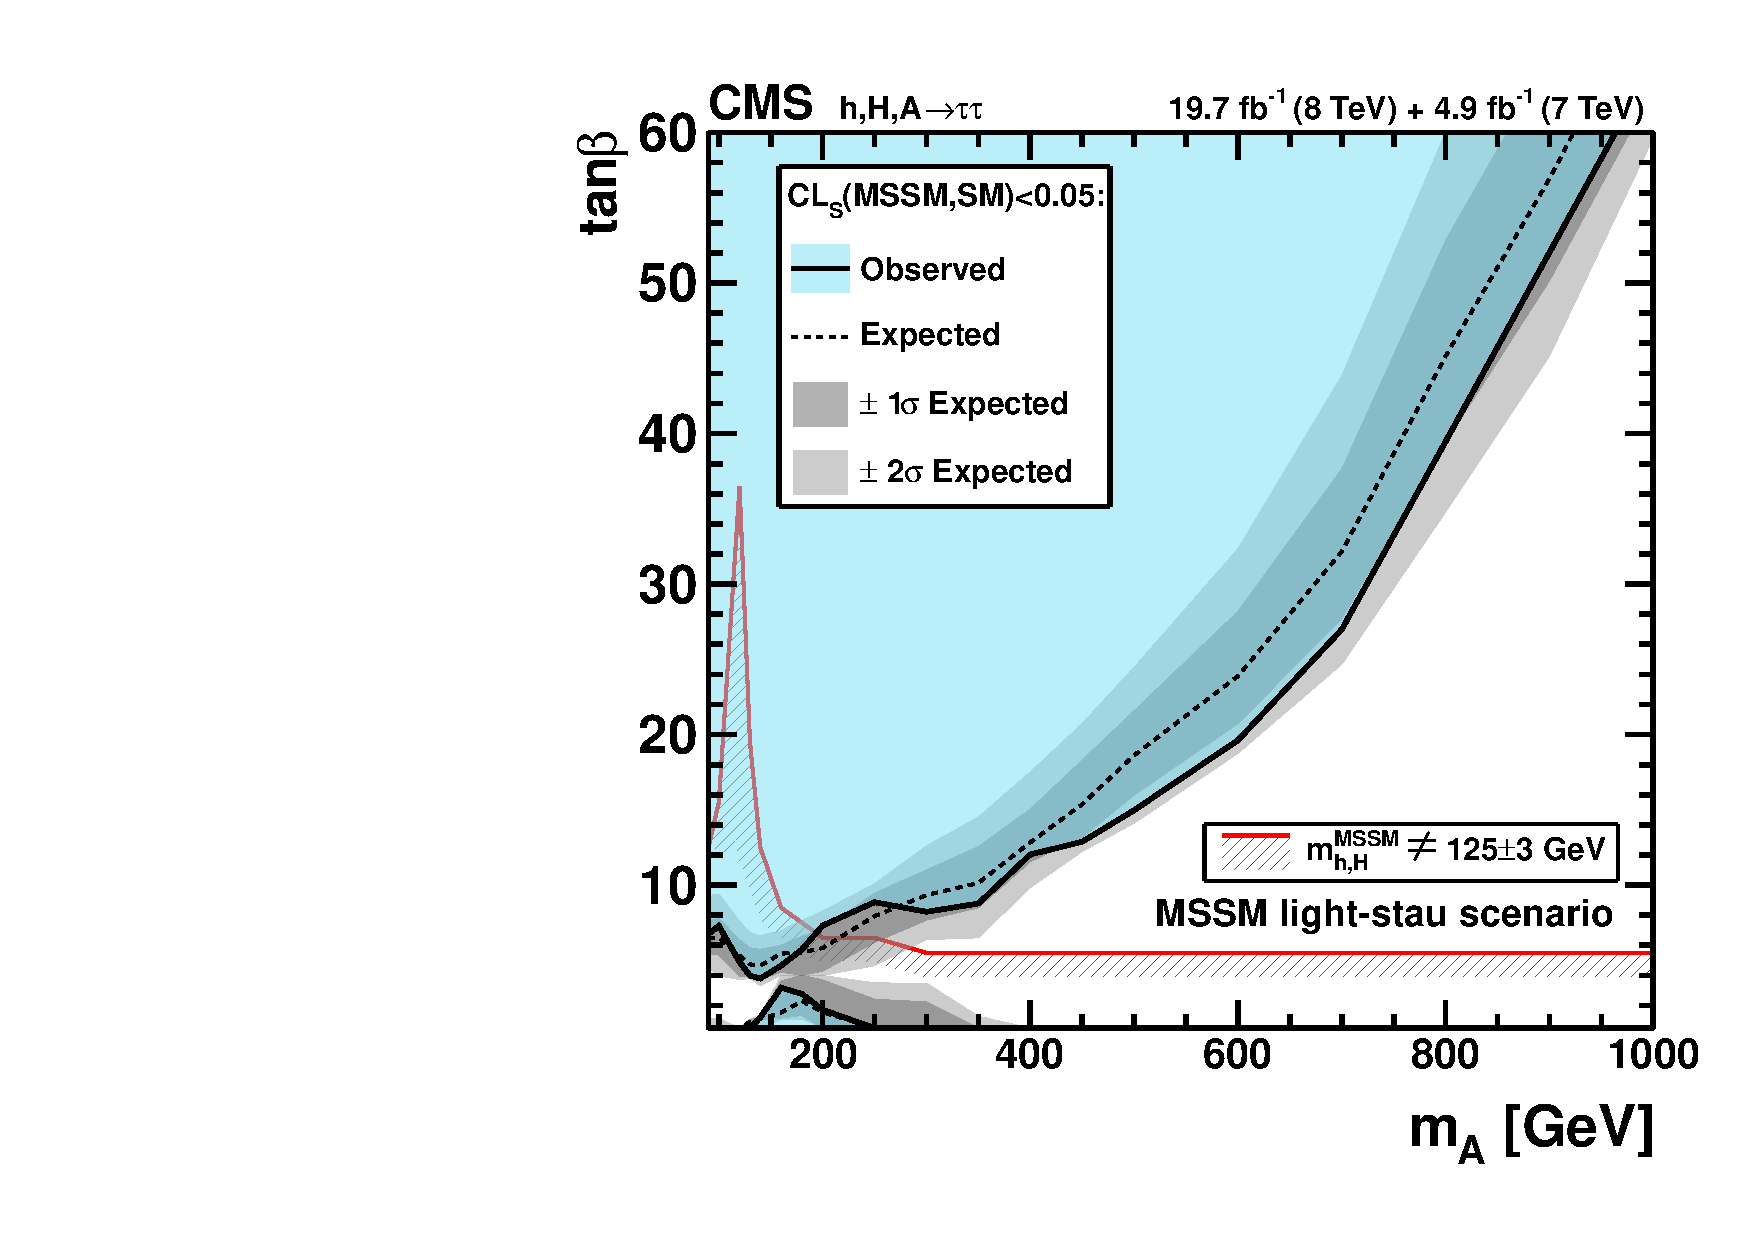
\includegraphics[width=0.5\textwidth]{plots/htt-mssm/cmbRL_lightstau1-HypoTest.pdf}}
\subfloat[]{
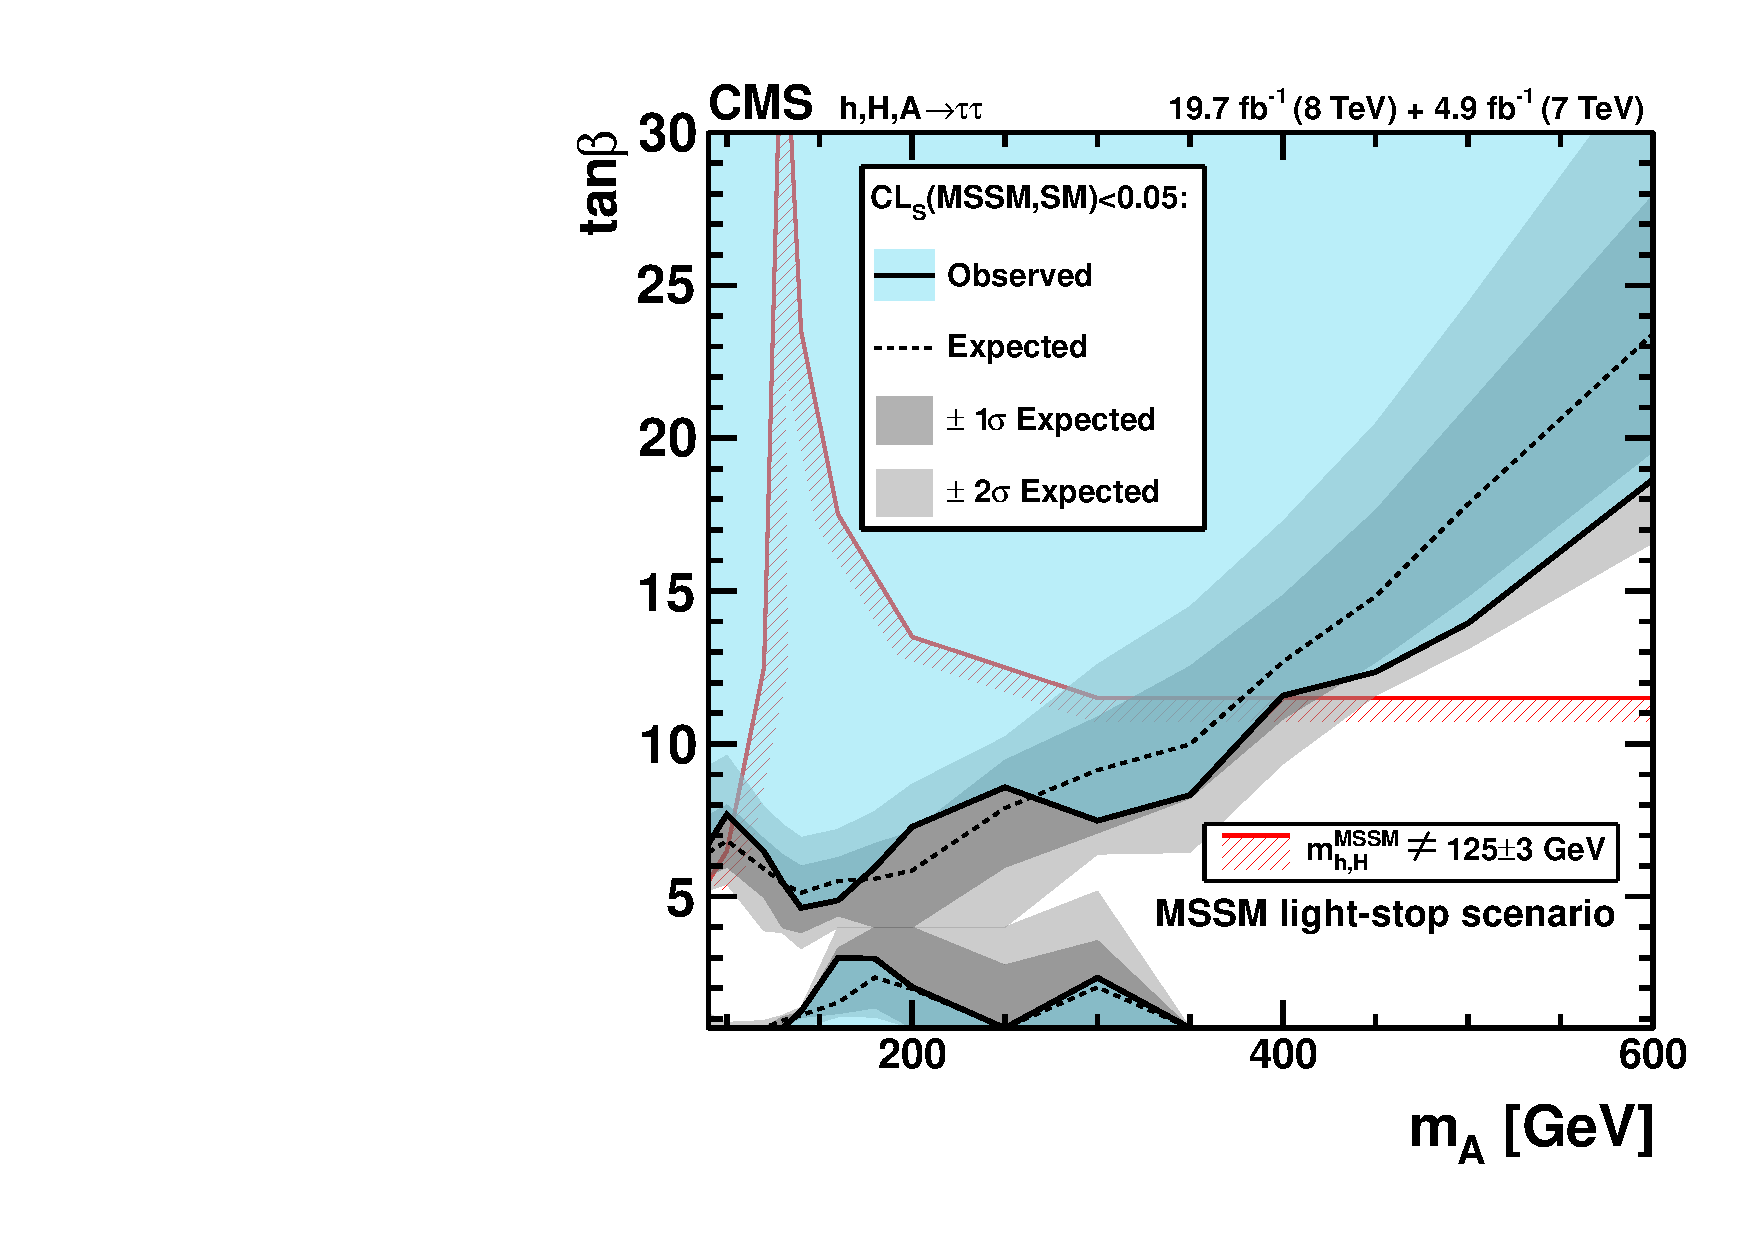
\includegraphics[width=0.5\textwidth]{plots/htt-mssm/cmbRL_lightstopmod-HypoTest.pdf}}
\caption[Expected and observed limit in the $m_{\PA}-\tan\beta$ plane of the
light-stau scenario (a) and light-stop scenario (b).]
{Expected and observed limit in the $m_{\PA}-\tan\beta$ plane of the
light-stau scenario (a) and light-stop scenario (b). Hypothesis
separation testing is used to compare the \ac{MSSM} hypothesis with the \ac{SM}
hypothesis. The red area indicates the region of phase space which is already
excluded by the Higgs mass constraint of $125\pm3\,\GeV$ \cite{HIG-13-021}.}
\label{fig:lightstaulightstop}
\end{figure}

\begin{figure}[tbh]
\subfloat[]{
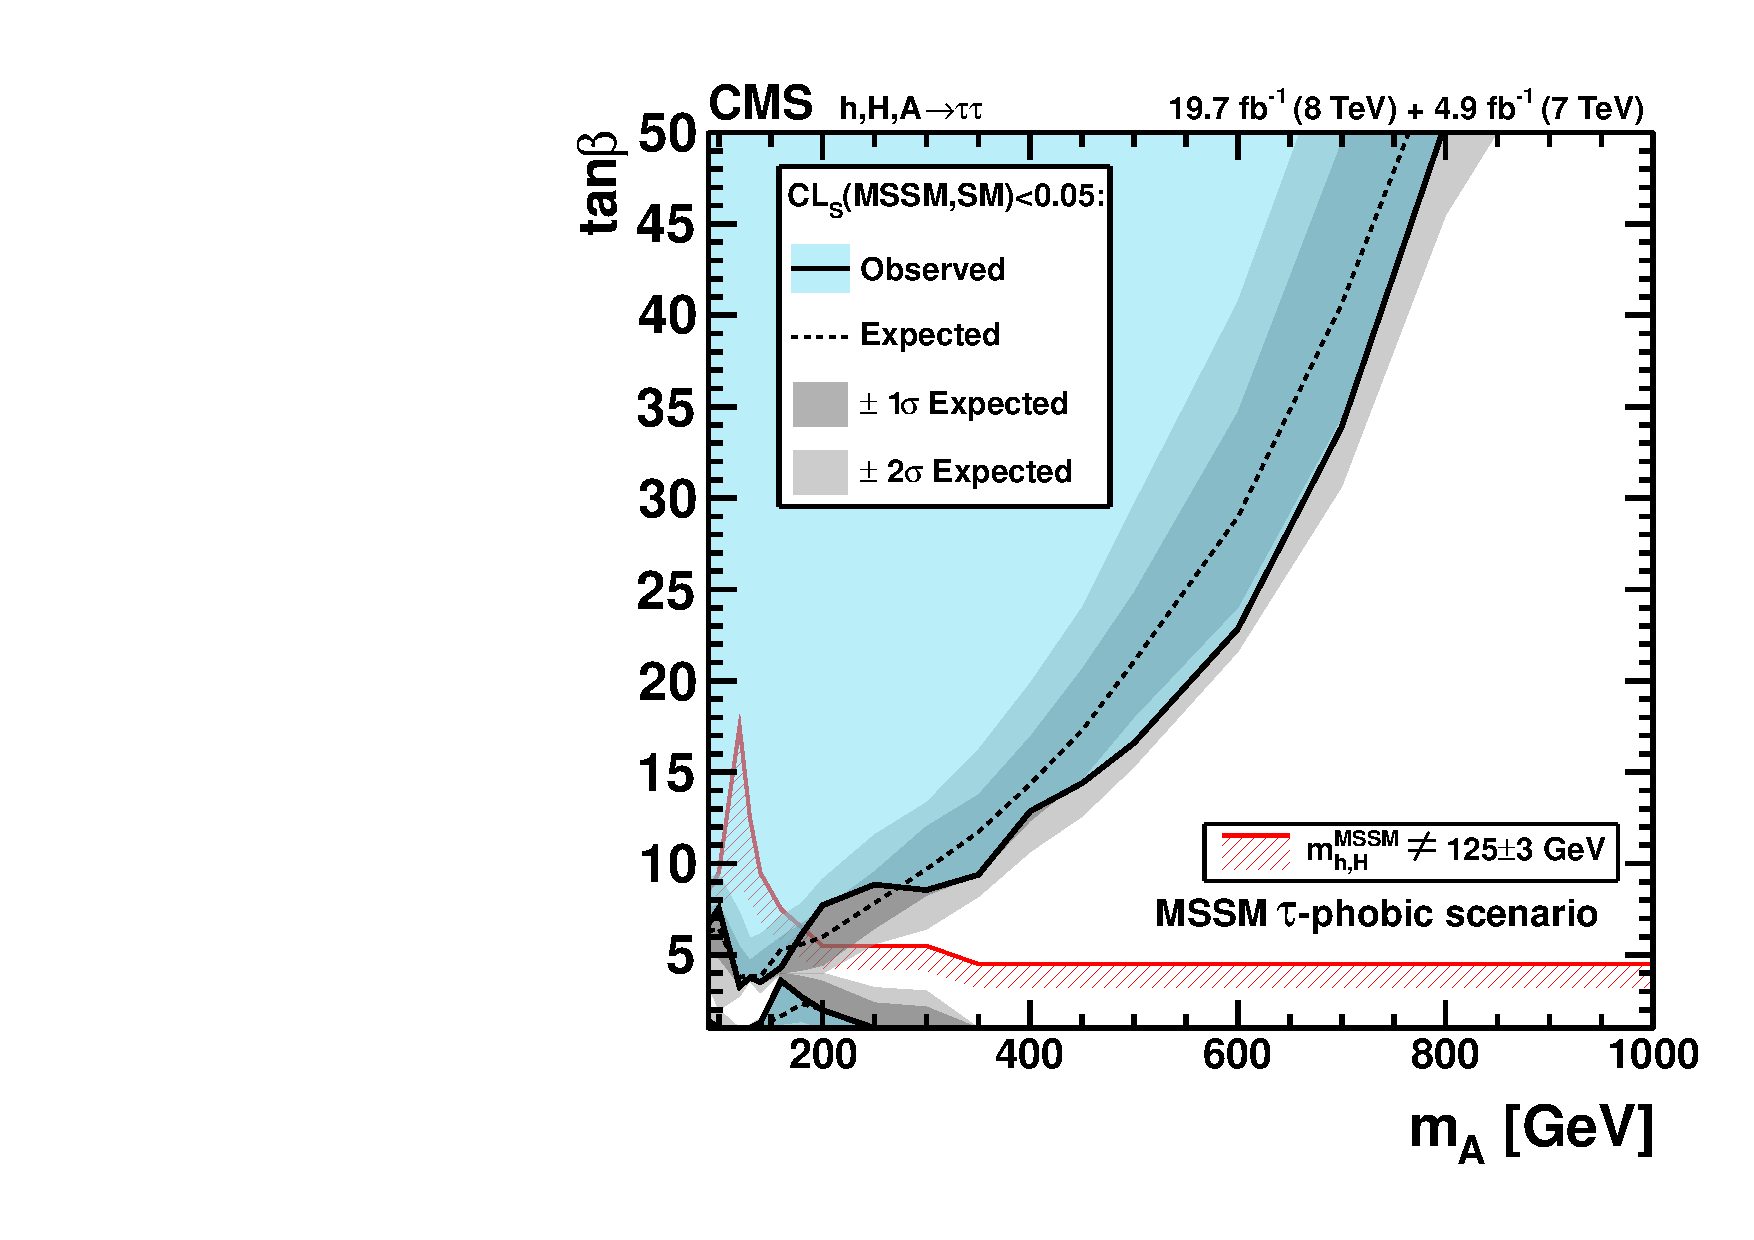
\includegraphics[width=0.5\textwidth]{plots/htt-mssm/cmbRL_tauphobic-HypoTest.pdf}}
\subfloat[]{
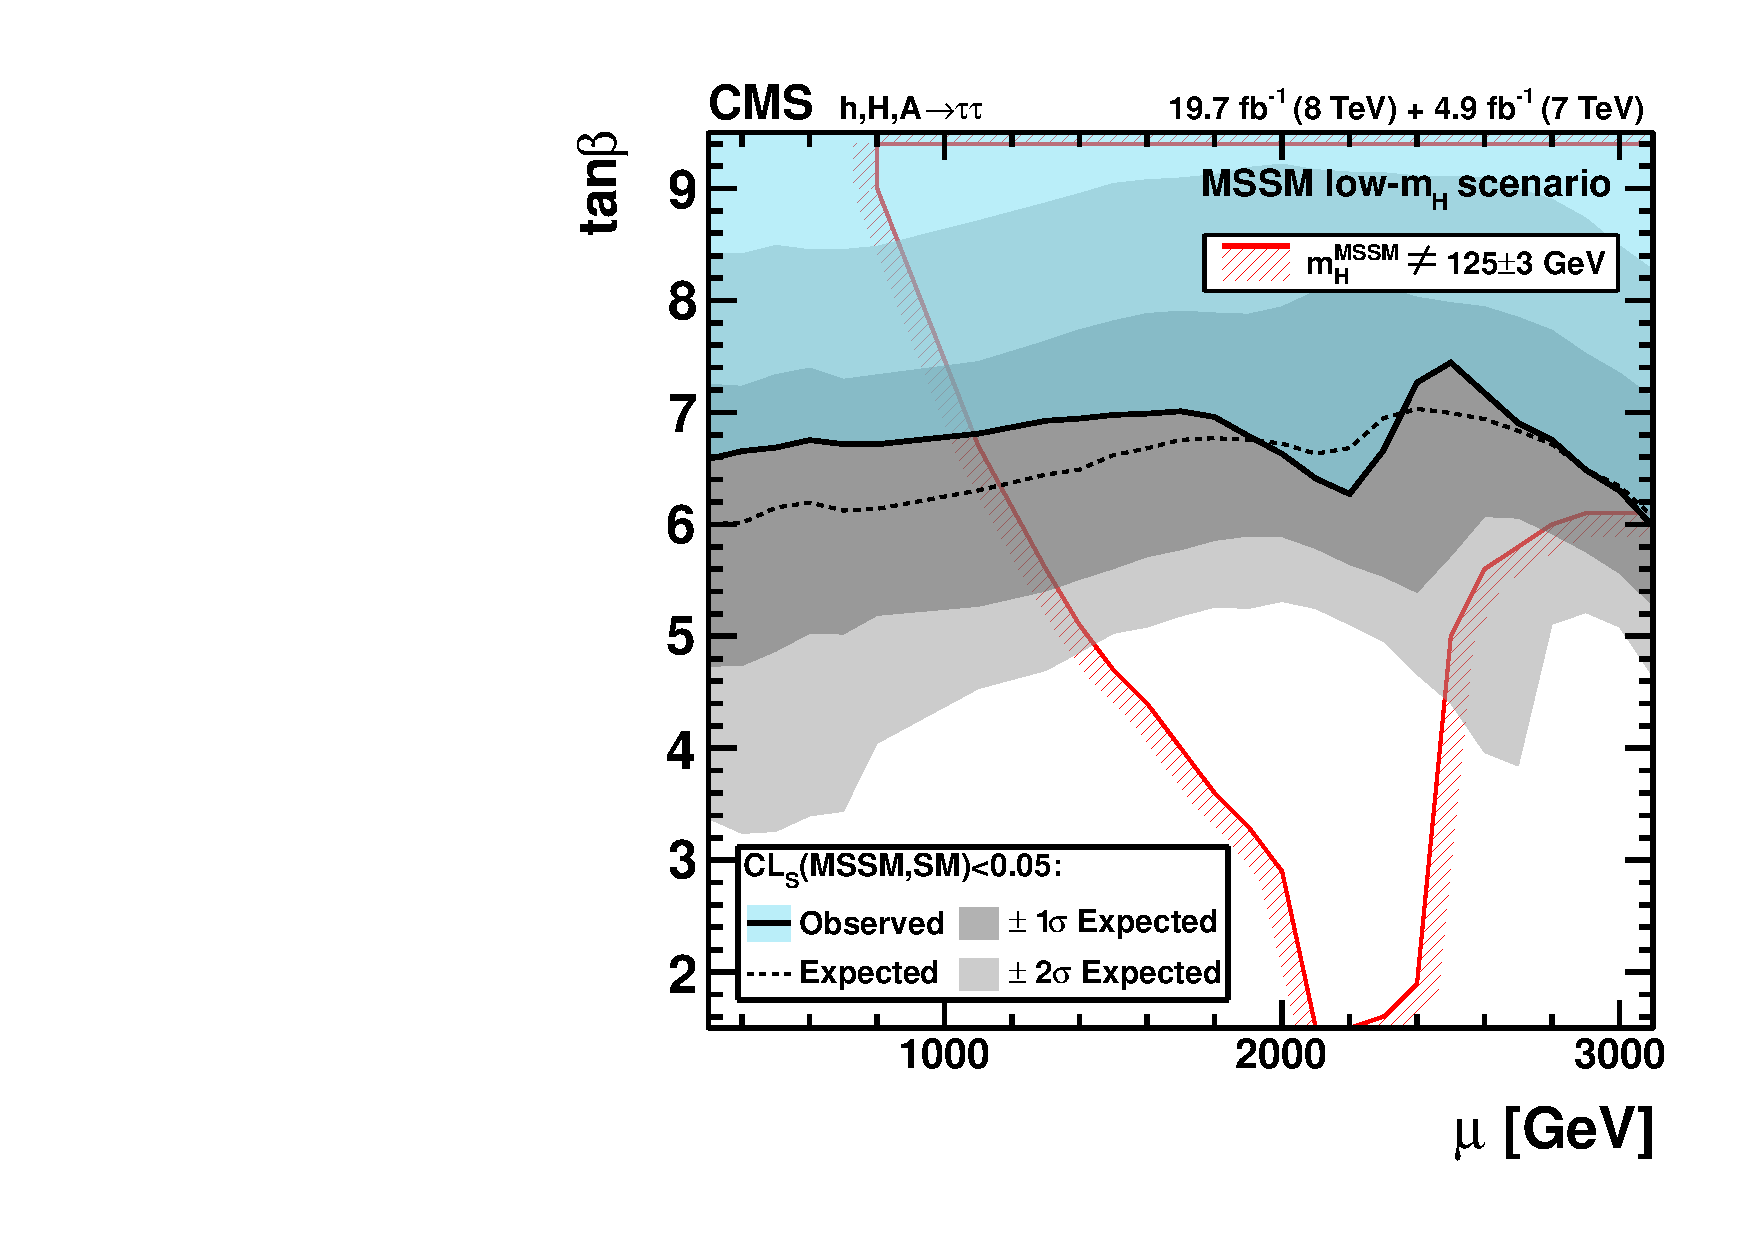
\includegraphics[width=0.5\textwidth]{plots/htt-mssm/cmbRL_lowmH-HypoTest.pdf}}
\caption[Expected and observed limit in the $m_{\PA}-\tan\beta$ plane of the
$\tau$-phobic scenario (a) and the $\tan\beta$-$\mu$ plane of the low-$m_{\PH}$ scenario (b).]
{Expected and observed limit in the $m_{\PA}-\tan\beta$ plane of the
$\tau$-phobic scenario (a) and the $\tan\beta$-$\mu$ plane of the 
low-$m_{\PH}$ scenario (b). Hypothesis
separation testing is used to compare the \ac{MSSM} hypothesis with the \ac{SM}
hypothesis. The red area indicates the region of phase space which is already
excluded by the Higgs mass constraint of $125\pm3\,\GeV$ \cite{HIG-13-021}.}
\label{fig:tauphobiclowmH}
\end{figure}
